%%% The main file. It contains definitions of basic parameters and includes all other parts.

%% Settings for single-side (simplex) printing
% Margins: left 40mm, right 25mm, top and bottom 25mm
% (but beware, LaTeX adds 1in implicitly)
\documentclass[12pt,a4paper]{report}
\setlength\textwidth{145mm}
\setlength\textheight{247mm}
\setlength\oddsidemargin{15mm}
\setlength\evensidemargin{15mm}
\setlength\topmargin{0mm}
\setlength\headsep{0mm}
\setlength\headheight{0mm}
% \openright makes the following text appear on a right-hand page
\let\openright=\clearpage

%% Settings for two-sided (duplex) printing
% \documentclass[12pt,a4paper,twoside,openright]{report}
% \setlength\textwidth{145mm}
% \setlength\textheight{247mm}
% \setlength\oddsidemargin{14.2mm}
% \setlength\evensidemargin{0mm}
% \setlength\topmargin{0mm}
% \setlength\headsep{0mm}
% \setlength\headheight{0mm}
% \let\openright=\cleardoublepage

%% Generate PDF/A-2u
\usepackage[a-2u]{pdfx}

%% Character encoding: usually latin2, cp1250 or utf8:
\usepackage[utf8]{inputenc}

%% Prefer Latin Modern fonts
\usepackage{lmodern}

%% Further useful packages (included in most LaTeX distributions)
\usepackage{amsmath}        % extensions for typesetting of math
\usepackage{amsfonts}       % math fonts
\usepackage{amsthm}         % theorems, definitions, etc.
\usepackage{bbding}         % various symbols (squares, asterisks, scissors, ...)
\usepackage{bm}             % boldface symbols (\bm)
\usepackage{graphicx}       % embedding of pictures
\usepackage{fancyvrb}       % improved verbatim environment
\usepackage{natbib}         % citation style AUTHOR (YEAR), or AUTHOR [NUMBER]
\usepackage[nottoc]{tocbibind} % makes sure that bibliography and the lists
			    % of figures/tables are included in the table
			    % of contents
\usepackage{dcolumn}        % improved alignment of table columns
\usepackage{booktabs}       % improved horizontal lines in tables
\usepackage{paralist}       % improved enumerate and itemize
\usepackage{xcolor}         % typesetting in color

\usepackage{float}			% allows to position images mor preciously.
%%% Basic information on the thesis

% Thesis title in English (exactly as in the formal assignment)
\def\ThesisTitle{Client-side execution of PHP applications compiled to .NET}

% Author of the thesis
\def\ThesisAuthor{Tomáš Husák}

% Year when the thesis is submitted
\def\YearSubmitted{2021}

% Name of the department or institute, where the work was officially assigned
% (according to the Organizational Structure of MFF UK in English,
% or a full name of a department outside MFF)
\def\Department{Department of Software Engineering}

% Is it a department (katedra), or an institute (ústav)?
\def\DeptType{Department}

% Thesis supervisor: name, surname and titles
\def\Supervisor{RNDr. Filip Zavoral, Ph.D.}

% Supervisor's department (again according to Organizational structure of MFF)
\def\SupervisorsDepartment{Department of Software Engineering}

% Study programme and specialization
\def\StudyProgramme{Computer Science (B1801)}
\def\StudyBranch{ISDI (1801R049)}

% An optional dedication: you can thank whomever you wish (your supervisor,
% consultant, a person who lent the software, etc.)
\def\Dedication{%
Dedication.
}

% Abstract (recommended length around 80-200 words; this is not a copy of your thesis assignment!)
\def\Abstract{%
\change[inline]{Write an abstract.}
}

% 3 to 5 keywords (recommended), each enclosed in curly braces
\def\Keywords{%
{PHP} {.NET} {Blazor} {Peachpie}
}

%% The hyperref package for clickable links in PDF and also for storing
%% metadata to PDF (including the table of contents).
%% Most settings are pre-set by the pdfx package.
\hypersetup{unicode}
\hypersetup{breaklinks=true}

% Definitions of macros (see description inside)
%%% This file contains definitions of various useful macros and environments %%%
%%% Please add more macros here instead of cluttering other files with them. %%%

%%% Minor tweaks of style

% These macros employ a little dirty trick to convince LaTeX to typeset
% chapter headings sanely, without lots of empty space above them.
% Feel free to ignore.
\makeatletter
\def\@makechapterhead#1{
  {\parindent \z@ \raggedright \normalfont
   \Huge\bfseries \thechapter. #1
   \par\nobreak
   \vskip 20\p@
}}
\def\@makeschapterhead#1{
  {\parindent \z@ \raggedright \normalfont
   \Huge\bfseries #1
   \par\nobreak
   \vskip 20\p@
}}
\makeatother

% This macro defines a chapter, which is not numbered, but is included
% in the table of contents.
\def\chapwithtoc#1{
\chapter*{#1}
\addcontentsline{toc}{chapter}{#1}
}

% Draw black "slugs" whenever a line overflows, so that we can spot it easily.
\overfullrule=1mm

%%% Macros for definitions, theorems, claims, examples, ... (requires amsthm package)

\theoremstyle{plain}
\newtheorem{thm}{Theorem}
\newtheorem{lemma}[thm]{Lemma}
\newtheorem{claim}[thm]{Claim}

\theoremstyle{plain}
\newtheorem{defn}{Definition}

\theoremstyle{remark}
\newtheorem*{cor}{Corollary}
\newtheorem*{rem}{Remark}
\newtheorem*{example}{Example}

%%% An environment for proofs

\newenvironment{myproof}{
  \par\medskip\noindent
  \textit{Proof}.
}{
\newline
\rightline{$\qedsymbol$}
}

%%% An environment for typesetting of program code and input/output
%%% of programs. (Requires the fancyvrb package -- fancy verbatim.)

\DefineVerbatimEnvironment{code}{Verbatim}{fontsize=\small, frame=single}

%%% The field of all real and natural numbers
\newcommand{\R}{\mathbb{R}}
\newcommand{\N}{\mathbb{N}}

%%% Useful operators for statistics and probability
\DeclareMathOperator{\pr}{\textsf{P}}
\DeclareMathOperator{\E}{\textsf{E}\,}
\DeclareMathOperator{\var}{\textrm{var}}
\DeclareMathOperator{\sd}{\textrm{sd}}

%%% Transposition of a vector/matrix
\newcommand{\T}[1]{#1^\top}

%%% Various math goodies
\newcommand{\goto}{\rightarrow}
\newcommand{\gotop}{\stackrel{P}{\longrightarrow}}
\newcommand{\maon}[1]{o(n^{#1})}
\newcommand{\abs}[1]{\left|{#1}\right|}
\newcommand{\dint}{\int_0^\tau\!\!\int_0^\tau}
\newcommand{\isqr}[1]{\frac{1}{\sqrt{#1}}}

%%% Various table goodies
\newcommand{\pulrad}[1]{\raisebox{1.5ex}[0pt]{#1}}
\newcommand{\mc}[1]{\multicolumn{1}{c}{#1}}

%%% User defined macors

%%% Coding packages for pseudocode 
\usepackage{listings}
\lstset
{
	frame=tlrb,
	numbers=left,
	breaklines=true,
	breakatwhitespace=true,
	tabsize=2,
	literate={\ \ }{{\ }}1
}

%%% Todo notes
\usepackage{xargs}	% Use more than one optional parameter in a new commands
\usepackage[colorinlistoftodos,prependcaption,textsize=tiny]{todonotes}
\newcommandx{\unsure}[2][1=]{\todo[linecolor=red,backgroundcolor=red!25,bordercolor=red,#1]{#2}}
\newcommandx{\change}[2][1=]{\todo[linecolor=blue,backgroundcolor=blue!25,bordercolor=blue,#1]{#2}}
\newcommandx{\info}[2][1=]{\todo[linecolor=OliveGreen,backgroundcolor=OliveGreen!25,bordercolor=OliveGreen,#1]{#2}}
\newcommandx{\improvement}[2][1=]{\todo[linecolor=Plum,backgroundcolor=Plum!25,bordercolor=Plum,#1]{#2}}
\newcommandx{\thiswillnotshow}[2][1=]{\todo[disable,#1]{#2}}


% Title page and various mandatory informational pages
\begin{document}
%%% Title page of the thesis and other mandatory pages

%%% Title page of the thesis

\pagestyle{empty}
\hypersetup{pageanchor=false}
\begin{center}

\centerline{\mbox{
\includegraphics[width=166mm]{./img/logo-en.pdf}}}

\vspace{-8mm}
\vfill

{\bf\Large BACHELOR THESIS}

\vfill

{\LARGE\ThesisAuthor}

\vspace{15mm}

{\LARGE\bfseries\ThesisTitle}

\vfill

\Department

\vfill

{
\centerline{\vbox{\halign{\hbox to 0.45\hsize{\hfil #}&\hskip 0.5em\parbox[t]{0.45\hsize}{\raggedright #}\cr
Supervisor of the bachelor thesis:&\Supervisor \cr
\noalign{\vspace{2mm}}
Study programme:&\StudyProgramme \cr
\noalign{\vspace{2mm}}
Study branch:&\StudyBranch \cr
}}}}

\vfill

% Zde doplňte rok
Prague \YearSubmitted

\end{center}

\newpage

%%% Here should be a bound sheet included -- a signed copy of the "bachelor
%%% thesis assignment". This assignment is NOT a part of the electronic
%%% version of the thesis. DO NOT SCAN.

%%% A page with a solemn declaration to the bachelor thesis

\openright
\hypersetup{pageanchor=true}
\pagestyle{plain}
\pagenumbering{roman}
\vglue 0pt plus 1fill

\noindent
I declare that I carried out this bachelor thesis independently, and only with the cited
sources, literature and other professional sources. It has not been used to obtain another
or the same degree.

\medskip\noindent
I understand that my work relates to the rights and obligations under the Act No.~121/2000 Sb.,
the Copyright Act, as amended, in particular the fact that the Charles
University has the right to conclude a license agreement on the use of this
work as a school work pursuant to Section 60 subsection 1 of the Copyright~Act.

\vspace{10mm}

\hbox{\hbox to 0.5\hsize{%
In \hbox to 6em{\dotfill} date \hbox to 6em{\dotfill}
\hss}\hbox to 0.5\hsize{\dotfill\quad}}
\smallskip
\hbox{\hbox to 0.5\hsize{}\hbox to 0.5\hsize{\hfil Author's signature\hfil}}

\vspace{20mm}
\newpage

%%% Dedication

\openright

\noindent
\Dedication

\newpage

%%% Mandatory information page of the thesis

\openright

\vbox to 0.5\vsize{
\setlength\parindent{0mm}
\setlength\parskip{5mm}

Title:
\ThesisTitle

Author:
\ThesisAuthor

\DeptType:
\Department

Supervisor:
\Supervisor, \SupervisorsDepartment

Abstract:
\Abstract

Keywords:
\Keywords

\vss}

\newpage

\openright
\pagestyle{plain}
\pagenumbering{arabic}
\setcounter{page}{1}


%%% A page with automatically generated table of contents of the bachelor thesis

\tableofcontents

%%% Each chapter is kept in a separate file
\chapter*{Introduction}
\addcontentsline{toc}{chapter}{Introduction}

We can divide web applications into two types by roles of server and client.
However, they use different technologies for their purpose.
We will start with common parts.
An internet protocol, HTTP, usually carries out the communication between a server and a client.
A client uses a web browser for requesting a server.
A markup language HTML is essential for describing a page's structure.
A browser is responsible for interpreting and rendering the page's content.
It is a web application's environment for further interaction.
The need to adjust content by different styles initiates standardizing CSS language, which enriches pages with a wide graphical content.
\par
The first type is server-based web applications.
A server prepares the page, makes additional computations related to the request, and sends it back to the client.
Having a business logic on a server-side is the main objective.
The most popular language for server-side scripting becomes PHP.
\change[inline]{Add a statistic for the popularity of PHP}
\par
The second type is client-based web applications, where major business logic is moved to a client's browser.
However, the combination of CSS and HTML is sometimes sufficient.
This type of application needs dedicated technologies, which allow manipulation with a page structure, reacts to on-page events, and controls the browser's behavior.
Many languages were enabling the manipulation, but they were not usually supported by most browsers like Google Chrome, Safari, Opera, and Mozzila.
The scripting language Javascript became a browser standard from these supports.
\par
However, Javascript is a powerful language.
There are language-specific features, which are harder replaceable by the language.
Despite the urge, many technologies like Silverlight, which runs C\# code in a browser, or Adobe Flash Player with Actionscript were deprecated due to insufficient support across the browsers.
There appeared a portable binary-code format for executing programs, WebAssembly (abbreviated WASM) \squarecite{1} in 2015.
WebAssembly aims to secure high-performance applications on web pages.
Interop with Javascript makes the format as powerful as the language.
The advantage of WebAssembly is a being compilation target for many programming languages.
Since December 2019, when the W3 Consortium has begun recommending WebAssembly, it is easy to migrate other languages to the browsers supporting this recommendation.
\par
Many projects use the WASM as a target of compilation.
For example, the project PHP in browser \squarecite{2}.
It enables running PHP script inside our browser using predefined Javascript API or standard tag for HTML script.
Another project is an open-source framework Blazor \squarecite{3} developed by Microsoft.
It provides a runtime, libraries, and interop with Javascript for creating dynamic web pages using C\#.
\par
\change[inline]{Add a statistic for popularity of .NET}
The .NET and PHP popularity led to the creation of the Peachpie compiler.
Peachpie \squarecite{4} tries to make use of the .NET platform and offers PHP compilation to .NET.
It is a modern compiler enabling interop between PHP and C\#.
\par
The project opens the PHP door to Blazor.
An integration between Peachie and Blazor can yield to following benefits.
A community of PHP developers is significant.
Thus, many PHP libraries apply to working with client's data, cooperation with databases, and other server tasks.
The possibility to migrate the language PHP together with its conventions to a browser will impact developing dynamic web applications due to the PHP community and the libraries.
It can join PHP and C\# developers to collaborate with their programming languages using a minimum knowledge of the integration.
Another interesting functionality of this idea is a full C\#, PHP, and JavaScript interop which offers more options for developers and future extensions.
\par
This thesis uses the compilation of PHP scripts to .NET in order to execute PHP in a browser powered by Blazor.
The approach tries to achieve two goals.
The first goal is to enable web development on a client-side with PHP.
There are not libraries supporting this integration.
The second goal is to design the support to offer a convenient way to combine a PHP code with a Blazor.   
\par
The first chapter addresses the analysis of related work, alongside descriptions of the technologies used in the integration.
The second chapter analyses running PHP on the client-side and other problems related to used technologies.
The third gives a detailed problem's solution.
There are examples that demonstrate how to use all aspects of the created solution in chapter 4.
In chapter 5, we can see benchmarks that explore the limits of the implementation and compare them with the already existing project.
And the last chapter relates to a conclusion of this solution.

\chapter{Existing technologies}

In this chapter, we will give a short overview of web application functionality. 
We will explore server-side scripting using PHP and client-side scripting using Javascript in order to obtain observations of user conventions for interaction with web applications.
Afterward, we will introduce WASM, followed by the existing project enabling to execute PHP in a browser.
We will give short information about the .NET platform and C\# language.
In the last sections, we will introduce Blazor and Peachpie.

\section{PHP}

The basic principle of obtaining a web page is a request-response protocol, where a client sends a request for the web page using an HTTP protocol and receives a response with requested data.
The protocol uses a dedicated message format for communication.
Statelessness is a typical characteristic, meaning that a server has to retain information about clients and add additional information to the messages in order to distinguish between the clients.
\par
Since the server contains business logic, a browser has to send necessary data for required actions by an HTTP message.
The data are usually encoded as a part of \ac{URL} or in the HTTP message body.
HTML presents a tag \texttt{<form>} that enables interaction with the web application by a web form.
Figure \ref{img01:php} contains an example of the tag.
\texttt{<form>} can contain other tags, which are displayed as various types of fields.
A user fills these fields, and the browser sends the data as a new request to the server.
We can specify how the data will be encoded.
\texttt{get} method is one of the basic ways.
It encodes the data as a pair of keys and its values to the query part of the URL.
There is an example of URL
\texttt{http://www.example.com/index.php?par1=hello\&par2=world}.
A query part begins with a question mark.
We can see parameter keys \texttt{par1} and \texttt{par2} containing values \texttt{hello} and \texttt{world}.
Another method is called \texttt{post}, which encodes it in the request body, which does not appear in the URL.
\par
Although PHP \squarecite{5} was originally designed for user page templating on a server side, it has been adjusted gradually to enable writing application logic.
PHP is an interpreted language maintained by The PHP Group.
\par
We will describe the language by using figure \ref{img01:php} as an example.
The script includes a header, which adds a proper beginning of an HTML document.
Then, it prints a \texttt{post} content together with a file content whenever the file \texttt{file} was obtained.
There is a form enabling to send information about a name and attach a file to the massage.
A browser sends the message to the server via \texttt{post} method when the form is submitted.
The request is handled by \texttt{index.php} defined in \texttt{action}.
In the end, the script includes a proper ending of the document by \texttt{footer.php}.
\par
\begin{figure}
\begin{lstlisting}
<?php
    include("header.php");
?>

<h1>Superglobal POST</h1>
<?php
    foreach($_POST as $key => $value) { ?>
    <p><?php echo $key; ?> => <?php echo $value; ?></p>
<?php } ?>

<h1>File content:</h1>
<p>
<?php 
    if($_FILES["file"])
    {
        echo file_get_contents($_FILES["file"]["tmp_name"]);
    }	
?>
</p>

<form action="/index.php" method="post">
    <label for="name">Name:</label>
    <input type="text" id="name" name="name"><br>
    <label for="file">File:</label>
    <input type="file" id="file" name="file"><br>
    <input type="submit" value="Submit">
</form>

<?php
    inlude("footer.php");
?>
\end{lstlisting}
\caption{An example of PHP code in file index.php.}
\label{img01:php}
\end{figure}
\par
As we can see, the PHP code interleaves the HTML code, which has appeared to be a helpful method for data binding.
We call the feature HTML interleaving, which allows inserting PHP code in \texttt{<?php ... ?>} tag.
These fragments do not have to form individual independent blocks of code closed in curly brackets, as the example demonstrates by using the \texttt{foreach} cycle.
An interpreter executes a script from top to bottom. Everything outside the PHP tag is copied into the body of the request.
\par
We do not see any specification of type next to variables.
This is because the type system is dynamic.
A variable represents just a reference to the heap.
Its type is determined during runtime. 
\par
PHP has superglobals \squarecite{6}, which are built-in variables accessible from all scopes of the script.
Following superglobals are relevant to the thesis.
The \texttt{\$\_GET} variable stores parsed query part of the URL.
The \texttt{\$\_POST} variable stores variables which are sent by post method.
The \texttt{\$\_FILES} variable contains information about uploaded files sent by a client.
The uploaded file is saved as a temporary file, and standard reading operations can obtain the content.
This is demonstrated in the previously mentioned example by \texttt{file\_get\_contents} function.
\par
\change[inline]{Maybe add information about SESSION.}
\par
The nature of the request-response semantic usually results in a one-way pass of the application.
After dealing with a request, the script is terminated, meaning that the request is sent, and variables are disposed.
One of the well-known design patterns relating to PHP is the Front controller.
Usually, the main script invokes other parts of the program, based on the request, to deal with it and send the response back.
The idea of this pattern can be shown in figure \ref{img01:php}.
In the beginning, we delegate header rendering to \texttt{header.php} script.
Then we render the body and include \texttt{footer.php}, which cares about the proper ending of the HTML page.
\par
We can divide code in several ways.
Global functions are the most notable characteristic of PHP despite wide-spread object-oriented programming.
They are defined in the global scope and accessible from anywhere.
The next option is an object inspired by object-oriented programming.
We can include a PHP code from other scripts.
They can be recursively included during runtime, where variables remain across the inclusion.
Scripts can be composed into a package, which another code can reuse.

\section{Javascript}
\change[inline]{Zmena jako v uvodu}

A client-side code needs to control the rendered page and access a web interface providing additional services in order to interact with a user.
\change[inline]{Zjistit jestli to je jisty, protahnout predchozi vetu.}
The interface is usually available from Javascript.
We will start with a description of loading Javascript in a browser.
We will introduce a page representation in a browser alongside page events.
In the end, we will present Javascript as a scripting language for the creation of a responsive web page.
\par
\change[inline]{Zminit Dom pred parsovanim. Prohlizec uchovava strukturu DOMu, DOM je stromecek... Skript muze pracovat jen s tim co je nad nim. }
The process of generating a web page follows several steps.
A browser parses the HTML line by line. If a script occurs, the browser starts to execute the code.
The order of processing is important for manipulation with an HTML structure.
This limitation can be solved by web events mentioned later, but
it is a convention to add scripts to the end of the body part after all HTML tags are parsed.
\par
We can image a web page as an XML tree.
Its nodes are tags or text fragments, and its edges connect nodes with their children.
One representation of this tree is Document Object Model (abbreviated DOM).
Each node is represented by an object with special parameters relating to HTML and CSS. 
The nodes can contain other nodes representing their children.
Afterwards, there is a document node representing the whole document together with its root node.
\par
Events are the most common method of how to react to changing a web page state.
Every event can have some handlers(listeners).
Whenever an event occurs, it calls all its listeners.
There are many event types, but we will mention the ones that are important for us.
HTML tags are the most common entities which can have some events.
\change[inline]{xtt onclick, onload}
For example, a button has an event onclick which triggers when a client clicks on the button as we can see in listing \ref{img02:javascript}. 
Other events can represent a state of a page like onload which fires when the whole HTML document is parsed.
\par
A browser provides more APIs valuable for the application, like fetching extra data from a server or local storage.
These APIs are mentioned as Web API \squarecite{7}.
\par
ECMAScript is a Javascript standard recommending across browsers.
It is abravieted as ES.
\change[inline]{relates -> vic urcujiciho}
We can see later an abbreviation ES2015 which relates to the ECMAscript version.
Javascript is a high-level language usually executed by a browser's dedicated Javascript engine but can also be run on a desktop.
\change[inline]{Node.js je jediny ?}
Node.js is an example of a Javascript runtime running outside a browser.
Listing \ref{img02:javascript} will be used to show the language in the simple scenario.
The page contains a button that invokes an alert with a second delay when a client clicks on it.
\par
\begin{figure}[H]
\begin{lstlisting}
<!DOCTYPE html>
<html>
    <head>
    </head>
    <body>
        <button id="alert">Click to alert</button>
        <script>
            var handler = function (arg) {
                var timer = new Promise((resolve) => {
                    setTimeout(resolve, 1000);
                }); 
        
                timer.then(() => window.alert("Hello world."));
            };  

            var button = window.document.getElementById("alert");
            button.addEventListener("click", handler);
        </script>
    </body>
</html>
\end{lstlisting}
\caption{A Javascript code.}
\label{img02:javascript}
\end{figure}
\par
\change[inline]{as well as zmenit k nejak jako like PhP}
At first glance, we can see the type system is dynamic as well as PHP.
\change[inline]{xtt window}
A window is an essential global variable, which is an object representing the browser window of the running script.
The window object consists of all defined global variables.
It also contains a document property, which is an API for manipulating the DOM tree.
We can see the usage of the document property in the example.
Javascript object is often used as a wrapper of Web APIs.
\par
Functions are first-class citizens in Javascript.
We can treat them as common variables.
Javascript supports an event-driven style that helps to react to events conveniently.
\change[inline]{listing ref pridat}
There is a handler assigned to the click event in the listing.
\par
\change[inline]{Maybe add a section about async functions. Compare it with PHP}
\change[inline]{ale umoznuje efektivni sychnroni spracovani}
Javascript is single-threaded, which can be confusing with its constructs for promises.
The promise is a structure representing an unfinished process.
These processes can be chained.
However, the structure can give an illusion of multi-threading. It uses the scheduler for planning the next task executed by the main thread.
\change[inline]{Popsat blokujici operaci long running tasks}
The single thread is critical for blocking operations which causes thread freezing.
\par
Web workers \squarecite{11} are a browser feature enabling to run the script in the background.
\change[inline]{Spojit dve vety}
There are wrapped as Worker objects.
The worker limitation is communication with UI thread only by handling message events. 
Messages have to be serialized and deserialized.
\par
\change[inline]{presssent vyhodit which will need. Spojit prvni vetu s druhou. Organizace kodu}
Javascript module is the last thing, which we will need to present.
It gathers a collection of code.
Global entities of this code can be exported to another script.
These exports make an API of the module.
The module's advantage is defining the API and hiding the internal code, which is not relevant for the user.
\change[inline]{kompiluje se modul ?}
\change[inline]{zminit ze se to pousti v sandboxu}
\section{WebAssembly}

\change[inline]{current's}
WebAssembly \squarecite{9} is a new code format that can be run in today's browsers. 
It has a compact byte format, and its performance is near to a native code. 
WebAssembly is designed to be a compiling target of popular low-level languages like C or C++ due to its memory model.
It results in the possibility to run other languages in a browser because its runtime is often written in C or C++. 
The advantage of this format is a similarity with Javascript modules ES2015 after compilation into a machine code. 
\change[inline]{within misto by}
This enables browsers to execute it by a JavaScript runtime. 
\change[inline]{its se vztahuje k browsers}
So its security is as good as a code written in Javascript. 
Because of the same runtime, WebAssembly can call Javascript and vice versa.
\par
\change[inline]{Nappsat ze to bude pravdepodobne pridana}
Thread \squarecite{10} support is currently discussed nowadays and appears to be promising.
After all, new versions of Google Chrome experiments with proper multi-threading support.
A replacement of multi-threading can be Web workers mentioned in Javascript section.
\par
Despite supporting to run WebAssembly in a browser, the browser cannot load it as a standard ES2015 module yet.
WebAssembly JavaScript API was created in order to be able to load a WebAssembly to a browser using JavaScript.

\section{PHP in Browser}

The project \squarecite{2} aims to use compiled PHP interpreter into WebAssembly, which allows evaluating a PHP code.
\change[inline]{Kurziva txtt}
\change[inline]{Obrazek specialized script block}
The page has to import a specialized module php-wasm. 
A PHP code is evaluated by writing a specialized script block or manually by JavaScript and API.
PHP can afterward interact with JavaScript using a specialized API.
At first glance, that might be a good enough solution, but they are several parts that can be problematic due to PHP semantics.
\change[inline]{Ze tam neni abstrakce serveru...}
The solution doesn't solve superglobals. 
This is reasonable because this is the server's job, but you are not able to get information about a query part or handling forms without writing a JavaScript code.
\change[inline]{Dvakrat navigate}
The next problem is navigating how a script can navigate to another script without an additional support code which has to be JavaScript.

\section{C\# and .NET 5}

\change[inline]{have to odstranit}
\change[inline]{.NET je zastitujici nazev pro skupinu technologii...}
We have to introduce the Common Language Infrastructure (abbreviated CLI) \squarecite{18} before diving into .NET.
CLI is a specification describing executable code and runtime for running it on different architectures.
CLI contains descriptions of a type system, rules, and the virtual machine (runtime), which executes specified Common Intermediate Language (abbreviated CIL) by translating it to a machine code. 
The virtual machine is named CLR (Common Language Runtime).
CIL's advantage is a compilation target of languages like C\#, F\#, and VisualBlasic, which gives us great interoperability.
\change[inline]{.NET standard zminit nakonec}
.NET Framework, .NET 5, and Mono are implementations of CLI.
Although there are many CLI implementations, they are usually referred to as .NET.
\par
.NET Standard represents API's specifications of .NET libraries across different implementations.
.NET Standard offers to specify minimum requirements for the code.
\par
.NET 5 \squarecite{17} is the lastest version of .NET Core, which is a cross-platform successor to .NET Framework.
From now on, we will refer .NET 5 as .NET, since it should be the only supported framework in the future.
.NET is an open-source project primarily developed by Microsoft.
It consists of many libraries, runtime for executing CIL.
\change[inline]{runtime a knihovny}
The libraries can represent whole frameworks like ASP.NET, which aims to web development.
A large collection of code is usually compiled into an assembly containing the code and additional metadata.
As assembly can represent either a library or an executable program.
\par
\change[inline]{runtime pro dalsi platformy}
Mono aims to mobile platforms. 
Recently, they started to support compilation \squarecite{12} into WebAssembly.
This support allows executing CIL inside browsers.
The compilation has two modes.
The first one is compilation Mono runtime with all using assemblies.
The second one only compile Mono runtime, which then can execute .dll files without further compilation of them into WebAssembly.
A consequence of these compilations into WebAssembly is enabling to call Javascript and WebAPI from C\#.
\par
C\# is a high-level language using strong typing and a garbage collector.
It has a multi-paradigm, but its common characteristic is the objected-oriented style.
These features cause that C\# is a good language for a huge project which needs discipline from developers to hold the code understandable and manageable.

\section{Blazor}
\change[inline]{popsat strukturu, pak jejich konkretni priklady, mentioned later vyhazet}
Blazor is a part of the open-source ASP.NET Core framework.
Blazor allows creating client-side web applications written in C\# language.
Blazor framework offers two hosting models \squarecite{13} which have different approaches to creating web applications. 
The first one is referred to as Blazor Server App and represents a server-side web application using specific communication between a client for better functionality.
The thesis uses the second model, which Microsoft refers to as Blazor WebAssembly App, enabling to move business logic to a client-side without using Javascript.
\change[inline]{enebliing moving podivat se}
\par
From now on, we will use Blazor App to refer Blazor WebAssembly App.
\change[inline]{popsat vice, co je hostovana}
The application can be hosted by a standalone project representing a standard ASP.NET Core web server.
\change[inline]{Nezminovat solution}
It will become useful for further server settings, and the proposed solution utilizes it.
The division enables a choice of a place for the implementation of business logic.
\change[inline]{Nezminovat kdyz je spatne pripojeni}
If there is a bad connection, we can move the majority of business logic to the client and use the server for connection to a database; otherwise, we can use the client only for rendering the page.
When we choose the template, there are two main projects to describe.
\par
The first one is a server, which serves the Blazor App to a client.
There is nothing special about the project expects a middleware, which provides the Blazor files.
A middleware is a segment of an HTTP request pipeline, which cares about some functionality related to processing the request.
\par
We will describe the second project (Blazor App) in figure \ref{img01:project} to explain basic entities and their interaction with each other.
\par
\change[inline]{pridat i server obdelnicek}
\begin{figure}[H]\centering
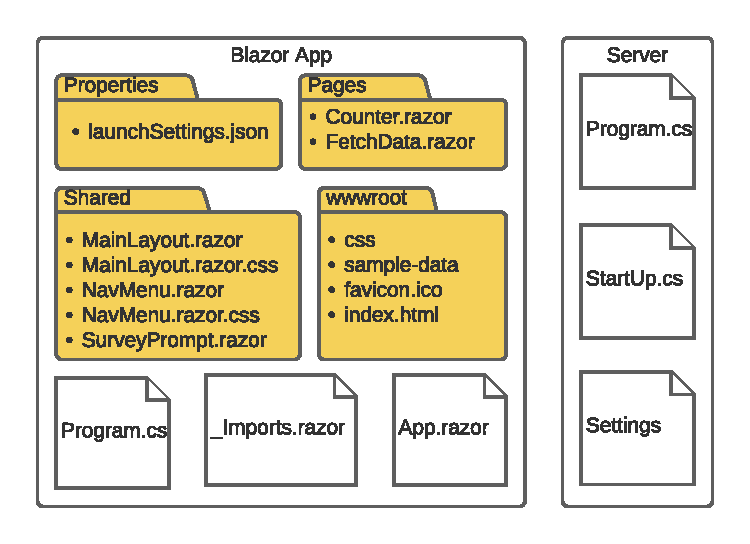
\includegraphics{./img/ProjectStructure}
\caption{A basic Web Assembly App project.}
\label{img01:project}
\end{figure} 
\par
We will start with a new format Razor to get familiar with it.
Razor is a markup language interleaving HTML with C\#.
Razor uses special sign at with keywords to identify C\# code in HTML.
Razor's compilation results in a pure C\# code representing the web page fragment.
We can see an example of Razor in listing \ref{img04:razor}.
\par
\begin{figure}
\begin{lstlisting}
@page "/example"
@inject HttpClient Http

<h1>Example</h1>
@if (!loaded)
{
    <p>Loading...</p>
}
else
{
    <p>Ticks: @ticks</p>
}

@code {
    private bool loaded = false;
    private int ticks = 0;

    protected override async Task OnInitializedAsync() {
        ticks = await Http.GetFromJsonAsync<int>("ticks.json");
        loaded = true;
    }
}
\end{lstlisting}
\caption{Example of Razor page.}
\label{img04:razor}
\end{figure}
\par
\change[inline]{zmenit point}
\change[inline]{if inject texttt}
Although the format is self-explaining, we point to the keywords.
The first line begins with a page keyword determining a part of the page's URL.
The next keyword is inject, representing a HttpClient service injection. 
An if keyword determines a standard condition.
\change[inline]{ridici struktura ktera se da prokladat}
A code keyword contains a regular C\# code, which can be used in the whole razor file.
\par
A Razor file is compiled into a C\# dedicated class.
The class inherits from ComponentBase or implements IComponent, which provides necessary methods for rendering the page.
Components can be arbitrarily put together in order to form the desired page.
We can see the generated Component from figure \ref{img04:razor} in figure \ref{img05:component}.
\par
\begin{figure}
\begin{lstlisting}
[Route("/example")]
public class Index : ComponentBase {
    private bool loaded = false;
    private int ticks = 0;
	
    [Inject] private HttpClient Http { get; set; }

    protected override void BuildRenderTree(
    							RenderTreeBuilder __builder) {
        __builder.AddMarkupContent(0, "<h1>Example</h1>");
        if (!loaded)
        {
            __builder.AddMarkupContent(1, "<p>Loading...</p>");
            return;
        }
        __builder.OpenElement(2, "p");
        __builder.AddContent(3, "Ticks: ");
        __builder.AddContent(4, ticks);
        __builder.CloseElement();
    }

    protected override async Task OnInitializedAsync() {
        ticks = await Http.GetFromJsonAsync<int>("ticks.json");
        loaded = true;
    }
}
\end{lstlisting}
\caption{Razor page generated to the C\# class.}
\label{img05:component}
\end{figure}
\par
We can assign the Razor keywords to parts of the code in the listing.
Page keyword stands for Route attribute.
Inject keyword stands for parameter attribute. The parameter is assigned by a dispatcher, mentioned later, during the initialization.
Code keyword is a part of class content.
Another markup is transformed into calling a specialized method in the BuildRenderTree function, which describes the page content for rendering. 
There will be more information about rendering later in this section.
\par
A Component has several stages, which can be used for initialization or action.
Virtual methods of ComponentBase represent these stages.
We can see the OnInitializedAsync method, which is invoked after setting the component's parameters.
\par
We should mention asynchronous processing because it helps render a page with long-loading content.
Blazor allows using Tasks and async methods.
\change[inline]{popis dvema vetama}
Blocking operations in Blazor are projected into UI because it is single-threaded due to Javascript and Web Assembly.
\par
We return to the project description. 
Folders Pages and Shared contains parts of Blazor pages written in Razor.
\_Imposts.razor contains namespaces, which are automatically included in others .razor files.
The next folder is wwwroot, containing static data of the application.
We can see index.html, which cares about loading parts of the Blazor application to the browser.
\par
\change[inline]{Add Static Web Assets}
\par
We will describe the loading of Blazor into the browser to fully understand the interaction between Blazor and the browser.
We have the server, the Blazor App, and other optional user's defined projects. 
When we start the server and tries to navigate the web application, the following process is done.
The server maps the navigation to index.html and sends it back.
\par
\change[inline]{odkaz a zmenit Javascript}
\begin{figure}
\begin{lstlisting}
<body>
    <div id="app">Loading...</div>
    <div id="blazor-error-ui">
        An unhandled error has occurred.
		...
    </div>
    <script src="_framework/blazor.webassembly.js"></script>
</body>

\end{lstlisting}
\caption{index.html}
\label{img06:index}
\end{figure}
\par 
The index.html contains a script initializing Blazor as we can see in figure \ref{img06:index}.
The first step is to load all resources, which are defined in a separate file.

Blazor cuts all unnecessary .dll files to reduce the size.
For this reason, all .dll has to be used in the Blazor App code in order to be contained in the file. 
These resources comprise Mono runtime compiled into WASM, additional supporting scripts, and all .dll files containing the whole application (Blazor App with referenced libraries).
The supporting scripts initiate the runtime a execute it.
The runtime includes the .dll into the application and calls the Main method in Program.cs defined in Blazor App project.
We can see the process in figure \ref{img07:wasm}.
\par
\begin{figure}[H]\centering
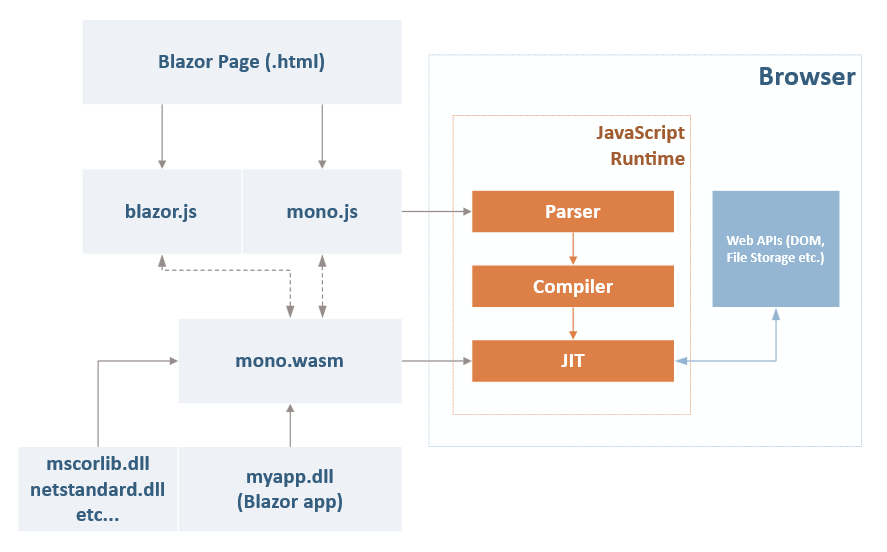
\includegraphics[width=140mm, height=100mm]{./img/BlazorExecution}
\caption{Running a Blazor WebAssembly App on client-side.}
\label{img07:wasm}
\end{figure}
\par
Main method uses WebAssemblyHostBuilder to set the application.
It defines services, which will be able through the dispatcher.
It set a root component, which will be rendered as the first.
The host is run.
Afterward, the application provides the dispatcher, cares about rendering, and communicates with the runtime to offer interop with Javascript.
\par
App.razor is the last file for clarification.
It is the root component in default.
It contains a specialized component, a Router, enabling to navigate the pages.
\par
In the end, we will describe page navigation and rendering and handling events.
\change[inline]{click on anchor...}
\change[inline]{Vymezit co dela blazor browser a javascript}
The navigation \squarecite{14} can be triggered by an anchor, form, or filling up the URL bar.
The URL bar is handled separatly by a browser.
JavaScript can influence the remainings elements.
Blazor App handles only an anchor.
After clicking on an anchor, a navigation event is fired.
One of the handlers is a javascript function, which invokes C\# method through Mono WASM. 
The method represents a navigation handler in Blazor App.
A user can add listeners to the handler, but the Router implements default behavior for navigating.
The Router finds out all components which implement an IComponent interface and tries to render the page according to path matching RouteAttribute of a component whenever the navigation is triggered.
It creates an instance of the class and fills in its parameters.
The Router calls BuildeRenderTree, which enables running the rendering process.
Previous created intences of components are disposed.
The navigation can be redirected to the server if there is no match.
\par
The rendering process begins with the Renderer initialized in the application's builder.
\change[inline]{virtual.. drzi si copii DOMU}
Renderer cares about representing a virtual DOM of the page, creating a page's updates, and updating it with the runtime interop's support.
Renderer provides RenderTreeBuider for describing page contents.
The builder provides an API for adding various types of content to Batch, which is a specialized structure for describing previous and present virtual DOM changes.
\change[inline]{Uhladit vetu, demanding performance}
The changes are recognized by a diff algorithm, which is used to reduce changing a DOM directly in a browser to its demanding performance.
\change[inline]{musi byt render tree uzpusobeny pro ten algoritmus}
The usage of RenderTreeBuilder is complicated due to the algorithm.
The purpose of Razor is to make an implementation C\# method BuildRenderTree easier.
When the Renderer prepares the Batch, it calls specialized Javascript API for changing the page through Mono runtime.
\par
\change[inline]{texttt RenderTreeBuiler}
The diff algorithm is used to minimize the browser's DOM  update after all components used RenderTreeBuilder to render their content.
This algorithm used sequence numbers for parts of HTML to identify modified sections.
Sequence numbers corespond to the order of RenderTreeBuilder's instructions in the source code.
A benefit of this information is detecting loops and conditional statements to generating smaller updates of DOM.  
\par
Event handling is just clever usage of the Renderer with dedicated Javascript API for updating, where the API registers the listener.
When the event is fired, the listener invokes C\# method representing the handler through the WASM runtime.
\par
\change[inline]{Prilepit k odstavci}
Blazor provides API for invoking Javascript functions and vice-versa.

\section{Peachpie}

Peachpie \squarecite{16} is a modern compiler based on Roslyn and Phalanger project.
It allows compiling PHP scripts into a .NET assembly, which can be executed alongside standard .NET libraries.
We will describe the basics.
\par
Because the languages have a different type system, Peachpie brings dedicated types for representing PHP variables in .NET.
Some of these types are PhpValue representing a standard PHP variable, PhpArray, or PhpAlias which is a reference to PhpValue.
\par
Another abstraction is the Context class.
We can imagine Context as a state of the script while it runs.
The Context consists of superglobals, global variables, declared functions, declared and included scripts.
It also manages input and output, where we can choose a resource.
The Context can also be considered as a configuration of the incoming script's execution.
All information about a request can be arranged to mock every situation on the server-side.
The possibility of saving the Context and using it later is a significant advantage used in the solution.
\par
\change[inline]{nesnazi, delat... tries}
Because some PHP libraries are written in C or C++, Peachpie tries to implement them using .NET libraries.
These libraries are created as a dedicated type of assembly presented by Peachpie.
Using this assembly can add additional functions, which can provide an extra nonstandard functionality such as an interaction with a browser.
\par
\change[inline]{jsou to normalni assemly, }
The main advantage of the compiler is the great interoperability between PHP and .NET.
An option to work with C\# objects, attributes, and calling methods will become crucial for achieving advanced interaction between Blazor and PHP.
\change[inline]{Saving script information in the assembly}
\change[inline]{Inheriting the CSharp classes}
\par
However, there are limitations following from differences in the languages and the stage of development.
Availability of PHP extensions depends on binding these functions to CSharp code which gives equivalent results. 
\change[inline]{Rozepsat. Oboustrane vyhoda, .NET knihovny nezavisle na prostredi bezi ve WabAssembly ale nemusi byt odladeny vykonostne}
The time and memory complexity of this code can be tricky in Blazor.
The previously mentioned interoperability has limits as well.
Csharp constructs like structs and asynchronous methods are undefined in PHP.
\change[inline]{V dobe psani prace tady byly nejake komplikace}

\chapter{Problem analysis}
We divide the analysis into three steps.
In the first section, we think of potential users of the integration in order to define realistic use cases for them.
Four use cases describe the user's intentions.
Then, we specify requirements, which are demanded by the use cases.
In the last section, we propose a high-level architecture of our solution, where we aim at utilizing Blazor and Peachpie to cover the requirements.

\section{Use Cases}
We remind technologies of interest to introduce a context of our use cases.
PHP is used for server scripting, where it is designed to process a request, create the website, and send it back.
Blazor is a web framework for creating a client-side UI using C\#.
Peachpie is a PHP compiler, which compiles a collection of PHP scripts, representing a standalone project, to a .NET assembly.
\par
A user persona \cite{online:persona} is a description of an imaginary user, which represents the needs of some group of users.
We use four user personas to cover use cases, which help us to identify requirements.
\par
The first persona is a C\# programmer, Blake, excited for Blazor.
He has already got acquainted with our solution.
\par
The second persona is a PHP programmer, Alice, who has no experience with Blazor but knows Peachpie basics.
Alice creates standard websites written in PHP, where she uses techniques introduces in the PHP section.
One day Blake tells her about our solution to migrate the scripts to a browser using Blazor and Peachpie.
She is excited by the solution and looks forward to using it.
However, she does not want to learn the Blazor framework.
\par
The third persona is a PHP programmer, Bob, who has already tried to write a simple website using Blazor and knows Peachpie basics.
He creates standard PHP websites similar to Alice's.
One day Blake tells him about our solution, and Bob's wish is to use the solution to help him inject his PHP scripts into Blazor websites.
Occasional work with the Blazor framework does not bother him, but it should have appropriate difficulty to his skills.
\par
The fourth persona is an enthusiastic PHP programmer, Chuck, who has advanced experience with Blazor and knows Peachpie basics.
He does not avoid exploring new technology to utilize all their aspects.
Blake tells him about our solution, and Chuck wishes that the solution offers him to collaborate with Blazor by PHP.
\par
These descriptions should help us determine the following use cases, which are realistic to them.
We call the first use case \textbf{Web} aiming at Alice.
We suppose she has a simple PHP website, which contains some information about her company.
The website does not work with a database and consists of pages containing images and references interconnecting them.
Some pages are adjustable by specifying the query part of the URL, and they include other scripts to add some basic layout.
One day the website notices many accesses, and Alice wants to migrate the website in order to a client side to save server resources.
The migration should download most of the website to a browser.
Afterward, navigation between scripts and script execution should be maintained on the client side.
Even more, Alice does not want to adjust the website for a client side too much, and she wishes for a simple solution that is understandable by a novice.
\par
We call the second use case \textbf{OneScript} aiming at Bob, who already has some experience with Blazor.
He wants to contribute to an existing Blazor website.
He has a great idea of adding a new widget, displaying the user's graph using HTML and CSS.
Because he is used to PHP, he wants to implement it with a few PHP scripts, which use some supporting libraries.
The idea consists of letting the user choose to load graph data from a file or generate a predefined graph as a demo.
After that, the widget renders HTML markup representing the graph.
Bob uses forms to interact with a user, and he is not willing to learn Javascript or interoperability between PHP and Blazor.
Thus, he needs a solution, which offers interaction with a user and uses standard PHP conventions mentioned earlier.
\par
We call the third use case \textbf{WebGame} aiming at Chuck.
He wants to create a real-time web game similar to Asteroids written in PHP.
He decides to target on a client side and utilizes Blazor, Peachpie, and our solution.
A client side execution should prevent network latency by loading the game in the beginning.
After that, the game will be independent of the network connection due to running the game and saving the game state by a browser.
PHP programmers have not been used to saving variables or defined functions across scripts because of the HTTP policy mentioned in the PHP section.
However, Chuck utilizes state persistent to saves a state of all game entities in variables.
Because he has previous experience with Blazor infrastructure, he will appreciate utilizing all Blazor aspects to run this game.
\par
\begin{figure}
\centering
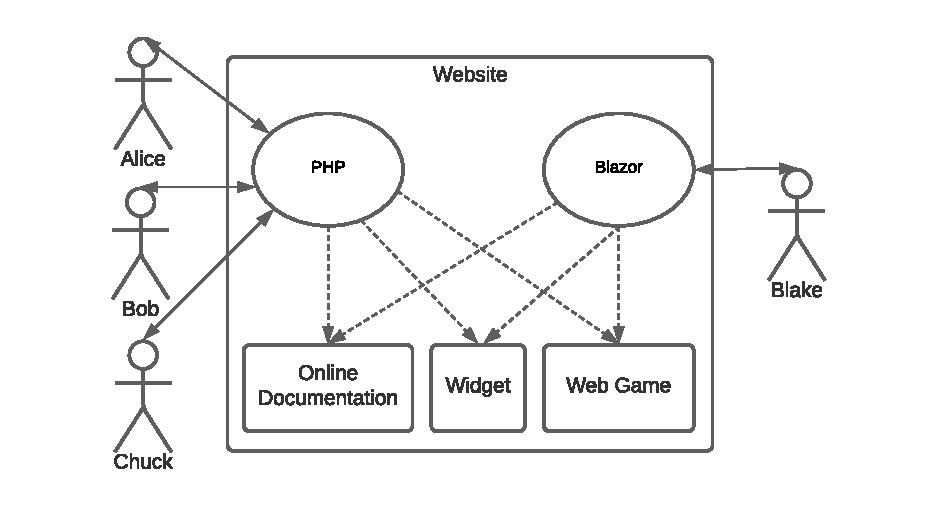
\includegraphics[scale=0.8]{./img/UseCaseAllTogether}
\caption{The \texttt{AllTogether} use case describing the combination of the all previous use cases. }
\label{img09:usecase}
\end{figure} 
\par
We can see an illustration of the fourth use case, which we call \textbf{AllTogether}, in Figure \ref{img09:usecase}.
A double-headed arrow represents the person's used language. 
A dashed arrow represents a possible usage, where the head aims at an implementation of a website part written in the language connected with that part.
The goal of the use case is to allow collaboration between PHP and Blazor programmers, where a difference of languages is not a barrier.  
We can image two teams creating a web application. 
They agreed on developing a client-side web application, where both teams aim at different parts of the website.
For example, one team wants to create a fun zone where a user can play some web game, we can imagine something like Asteroids, and the second team wants to create some online documentation about the game and the widget for the graph representation displaying a user's score.
Because Blazor targets client-side web applications, they want to utilize Blazor.
Unfortunately, these teams use a different favorite language, where the first team uses PHP and the second team uses C\#.
Even more, these teams want to contribute to any part of the Blazor website, meaning that doing the fun zone can be handled by either the C\# or PHP team.
They need some environment where the PHP team can code alongside the Blazor team, and they can focus on an arbitrary part of the web application.
We can see the intention in Figure \ref{img09:usecase} where each team can create a part aiming at the web game, the online documentation, and widget.
We can see the PHP team consists of Alice, Bob, and Chuck, having different skills with Blazor, so the environment should reflect it.
Even more, Blake should be able to manipulate their part of the application to customize it using C\#. For example, he should change the layout of the website without complex refactoring. 

\section{Requirements}

The goal of this section is to describe requirements based on mentioned use cases.
If the proposed solution covers the requirements, then PHP scripts will become a valuable part of a Blazor website.
\par
\textbf{Navigation} is the first requirement that our solution should provide.
We demonstrate navigation posibilities in Figure \ref{img10:scripts}.
Basic functionality should provide script routing, which finds a script by its name, executes it, and displays the output in a browser.
This intention is illustrated by the first rectangle containing a collection of scripts in the figure.
The solution should offer a straightforward router making a PHP website accessible, as we can see in the figure.
The simplicity is a necessary condition for the \textit{Web} use case and should be reflected.
Blazor should navigate components defined in \textit{script.php} due to the \textit{WebGame} use case, which uses Blazor structures.
\par
\textbf{Reusability} of script is an important feature to make the \textit{OneScript} use case more useful.
Thus, Bob can insert the widget in different parts of the website, meaning that he can create a new web page containing some content and insert the widget into it, as we can see in Figure \ref{img10:scripts} where the Blazor component is generated from a PHP script and a Razor file.
\par
\begin{figure}
\centering
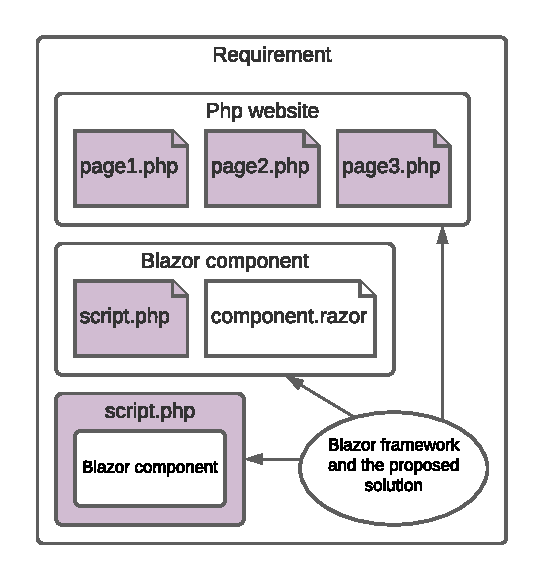
\includegraphics{./img/Requirement}
\caption{The requirement describing navigation between different types of entities. 
The proposed solution with Blazor connects these types into a single website, where they can live together.
}
\label{img10:scripts}
\end{figure} 
\par
\textbf{Interactivity} with a user is necessary in the \textit{WebGame}, and \textit{OneScript} use cases.
The solution should enable using common conventions in PHP, like forms, and be able to utilize Blazor features providing the interaction as well.
\par
\textbf{Rendering} should be maintained in two ways.
The first way aims at the \textit{Web} use case when a script output is transparently displayed as a web page or its fragment.
The approach hides Blazor infrastructure for rendering a markup and makes creating a UI easier for PHP programmers.
The second way aims at the \textit{WebGame} use case when the solution provides an interface for the interaction with Blazor.
It is also necessary when we want to use already defined components in a PHP code.
The rendering should be effective due to the high frame rate of the game.
\par
\textbf{State preservation} should be available for creating a web application by a collection of scripts saving their variables after the execution.
This feature is not typical for PHP because of PHP policy and conventions, where programmers are used to deletion of variables and function definitions after the request termination.
The state described by the variables needs to be preserved in order to interact with a user in a client-side application. 
For an example, the \textit{WebGame} use case uses variables to save the game state. 
However, we have to distinguish these situations where the feature is necessary.
\par
\textbf{Server simulation} should be the main advantage of the solution.
We could see superglobals are commonly used methods how to obtain information about navigation or submitted data.
The solution should support superglobals for examples like the \textit{Web} use case, where the website uses information about URL query part, via \texttt{\$\_GET} variable, to make decisions.
\par
\textbf{Forms} should be maintained by the solution. 
The forms are usually sent to a server, but the solution should handle them on a client side, where they should be provided to PHP scripts.
After navigation to a script defined in the \texttt{action} attribute, the script should access the form data.
We can upload files by form.
Thus, the solution should provide file management accessing and downloading them.
\par
\textbf{Interoperability} between PHP, Blazor, and Javascript should be supported for situations when forms, the server abstraction, or Blazor are not sufficient.
We need some representation of Blazor in PHP, which the \textit{WebGame} use case will use for interacting with a Blazor.
Javascript is essential for client side applications, and we should be able to use its features.

\section{Architecture}

The basic principle of our solution consists of PHP scripts compilation into .NET assembly by Peachpie.
After that, a Blazor App references \texttt{Peachpie.Blazor}, which is a support library providing a mechanism for navigating and executing the scripts.
Then, a server provides the application to a browser, where Mono runtime executes it.
We will describe the architecture from the view point of compilation time and runtime.
\par
When we think about PHP script compilation, there are two possibilities.
We can compile the scripts ahead of time and reference them from a Blazor App. 
The second way is to regard the scripts as Static Web Assets and load them into a browser as separated files.
Afterward, the Peachpie compiles and executes them.
Both approaches have different advantages. 
Thus, there is no silver bullet.
The first approach saves time by ahead compilation and compilation check.
However, the second approach can save browser memory when the web application is larger, and a client uses only a part of it.
We are inclined to the first approach because the static compilation is a standard way in Peachie.
We think that the first approach is valuable for the use cases mentioned earlier.
The \textit{Web} use case wants to save additional requests. 
The rest of the use cases intends to utilize small amounts of PHP scripts as a part of the website, so we suppose that the smaller size of resulting scripts is insignificant in contrast with the compiled Peachpie assembly, containing all of them. 
\par
We have to figure out how to attach a PHP code, which is compiled into the assembly, to the Blazor App.
Although Peachpie supports calling functions written in PHP from Blazor by default, we want to create an abstraction over the Blazor environment in order to simplify the interface.
The abstraction should offer a representation of PHP scripts in Blazor.
It should allow an option for accessing the Blazor interface for advanced features.
It should be compatible with the Blazor environment in other to allowing a smooth collaboration between the abstraction and the Blazor pages.
A Blazor page consists of components, which can collaborate with each other.
Thus, we can utilize them to represent PHP scripts.
Components can be arbitrarily put together, which offers to place our PHP code in the desired place in the Razor code.
Even more, we can replace a root component, \texttt{Router} by default, with the component representing PHP scripts.
Afterward, scripts will compose the whole Blazor website content.
The component provides a sufficient Blazor interface for rendering control and interaction with a browser. 
\par
We can think about how to represent PHP scripts as components.
We can consider one type of component, which will provide the abstraction for all the PHP code in scenarios.
A problem with this approach is that the use cases need different levels of abstraction.
The \textit{WebGame} use case wants to use the component for offering the Blazor interface accessible from PHP code.
The offer should contain identical or similar options, which are given in a C\# code.
The \textit{OneScript} use case wants to free a programmer from Blazor.
Thus, we want to use the component as an adjustable provider finding and executing PHP scripts.
Its purpose is to keep the user away from knowing about the detailed structure of Blazor and the integration.
Another important thing is a provider role in a Blazor App.
The provider can behave either as default Blazor \texttt{Router} or as a routable component, which enables the navigation of PHP scripts.
As a consequence, we need to create more types of components providing abstractions for the particular use cases.
However, only one type of component can manage all provider roles due to their similar rendering transparency.
The solution will reach two types of components.
The first one wants to bring Blazor to PHP in order to utilize the whole environment.
The second one aims at presenting a transparent execution of standard PHP script without knowing about the connection between Blazor and PHP.
We can illustrate out intention in Figure \ref{img12:component}.
\par
\begin{figure}
\centering
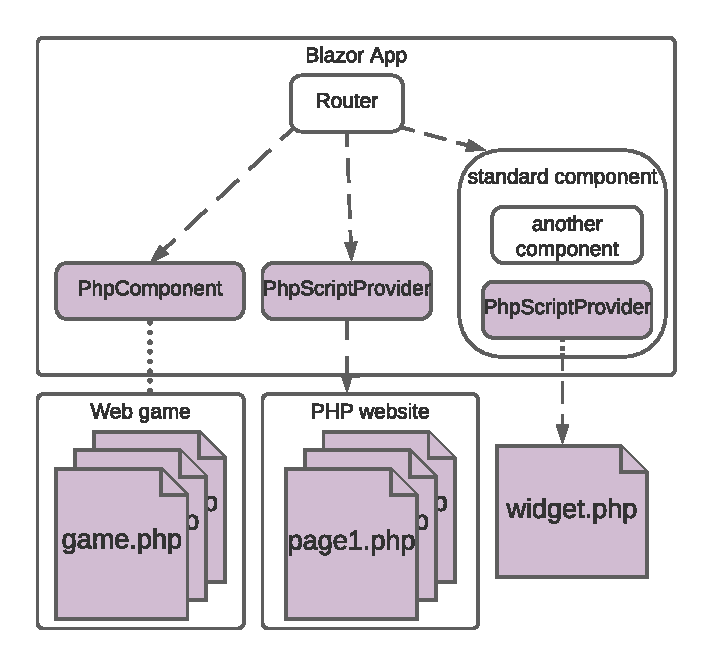
\includegraphics[scale=0.9]{./img/Components}
\caption{Components representing PHP scripts. Arrows represent navigation. 
Dot lines connect a runtime object with the implementation.
}
\label{img12:component}
\end{figure} 
\par
We will focus on the first component, which we will call \texttt{PhpComponent} due to the effort of moving the component concept to PHP.
\texttt{PhpComponent} aims at the third use case.
Despite language differences, we can utilize the common concept of classes and inheritance because Peachpie allows inheriting C\# class in a PHP code.
This feature results in full support of component interface without creating new structures for managing component behavior from PHP.
We can inherit \texttt{ComponentBase} class in PHP and use its methods in the same way as C\# class.
The inheritance offers the required interface in the \textit{WebGame} use case.
At the time of writing, there are also subproblems with the differences of languages.
The current Peachpie version does not support some C\# specifics fully.
The reason can be a hard or impossible representation of C\# entities in PHP.
We should develop some PHP support to enable using the parts of the Blazor interface, which can not be used in PHP directly.
\par
We will call the second type of component \texttt{PhpScriptProvider} expressing an environment for executing standard PHP scripts.
\texttt{PhpScriptProvider} solves the requirements of the remaining use cases \textit{Web}, \textit{OneScript}, and \textit{AllTogether}.
The provider should be able to navigate and execute PHP scripts.
Because the remaining use cases try to hide the integration between PHP and Blazor, the provider should support the following features.
It should pretend a server behavior, which copies everything in the output of PHP script to an HTTP response body rendered by a browser.
Superglobals are often used for obtaining additional information given by the user.
Thus, an ability to fill \texttt{\$\_GET} variable with the URL query part is important.
It should change a standard form functionality, which is sending the form to a server, to save the form information into superglobals, and executing the script again.
We target to load and save files submitted by form transparently in order to provide similar comfort to execute the script on a server side.
A possibility of saving the script context to the next execution is a new opportunity how to keep an application state in PHP script.
We will describe the provider modes.
These modes are intended to solve \textit{Web}, \textit{OneScript}, and \textit{AllTogether} use cases. 
\par
We call the first mode \textbf{Router}, which aims at the \textit{Web} use case, where the implementation is inspired by a GitHub project \cite{online:customRouter}.
It enables to set the provider as a root component.
It handles all navigation events, determines the script name, finds it, and executes the script.
Components defined in PHP code can also be navigation targets.
\par
We call the second mode \textbf{Script}, which aims at the \textit{OneScript} use case.
It enables the provider insertion into a Razor page.
Afterward, the provider executes the specified script.
\par
We call the third mode \textbf{ScriptProvider}, which aims at the \textit{AllTogether} use case.
It enables to navigate the set of scripts with respect to URL.
The navigation is generally maintained by the default \texttt{Router}.
The component only provides navigation to scripts.
\par
These observations lead us to make sure having two different components are rational ways how to separate the problems and offer an understandable difference between the components.



\chapter{Solution}

This chapter describes the complete solution, covering the use cases.
We start with an overview of the solution parts.
Then, we give a detailed description of each part.
\par
The proposed solution is implemented in \textit{Peachpie.Blazor}, which is a RCL library containing components mentioned in the previous section with an additional support code.
It is provided as a NuGet package containing an API for including PHP scripts to the website.
It defines a collection of support classes representing HTML entities, which makes the rendering easier.
A part of the support code is a Javascript script, which is linked to the beginning of the HTML document, providing helper functions for form handling and interoperability with PHP.
Then, the resulting Blazor website consists of three projects forming a .NET solution.
In Figure \ref{img13:infrastructure}, we can see these projects as green rectangles.
The \textit{Server} project references \textit{Blazor App}, containing a part of the website, and \textit{Peachpie.Blazor} library, containing the support code.
The server cares about providing the Blazor website and its Static Web Assets.
There is the \textit{Blazor App} project, which becomes the environment for running PHP scripts in a browser.
The rendering process and website composition, where the scripts are evaluated, are meant by the environment.
The project references the Peachpie project containing the programmer's PHP scripts and \textit{Peachpie.Blazor}, which content is used to maintain the scripts.
\textit{Blazor App} inserts the scripts using the components defined in the library.
\par
\begin{figure}[!b]\centering
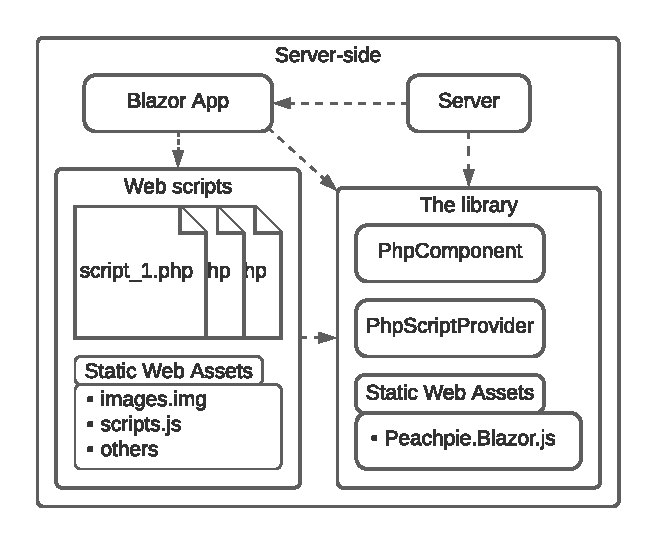
\includegraphics[scale=0.9]{./img/SolutionInfrastructure}
\caption{The solution infrastructure. Green rectangles represent projects. The orange rectangle represents a NuGet package. Arrows represent references.}
\label{img13:infrastructure}
\end{figure} 
\par
The first section aims at the server settings providing a Blazor application using PHP scripts and the \textit{Peachpie.Blazor} library.
The second section talks about \texttt{PhpComponent}.
It describes the resulting implementation and solutions of problems, which occurred during the implementation.
The last section aims at \texttt{PhpScriptProvider}.
It suggests a convenient way how to include the scripts into a browser, and it presents the component design.

\section{Server}

We have to set the server in order to provide additional static resources contained in a Peachpie project containing PHP scripts because the WebAssembly SDK ignores the \textit{wwwroot} folder of libraries except for RCL.
Thus, we create the \texttt{UseAdditionalWebStaticAssets} extension method of \texttt{IApplicationBuilder}, which inserts middlewares providing the resources into the request pipeline.
Its parameter is a configuration obtained from \textit{appsettings.json}, which is a part of the \texttt{BlazorApp.Server} project.
We can see an example of the configuration file in Figure \ref{img19:settings}, which defines a path to a folder and a base path used as a prefix of HTML document references.
Afterward, these resources can be referenced by URLs and downloaded from the server.
For example, we can reference an image with the path \texttt{WebGame/PHPScripts/wwwroot/image.jpg} as \texttt{/Asteroids/image.jpg} in HTML document on the client side.
Javascript helpers of our library can be found in the \textit{wwwroot} folder, which is transparently provided to a client side due to an RCL library type and the SDK.
\par
\begin{figure}[H]
\begin{lstlisting}
{
	...
  "AdditionalStaticWebAssets": [
    {
      "Path": "An//Absolute//Path//To//Resources//Directory",
      "BasePath": "/Asteroids"
    }
  ]
  ...
}

\end{lstlisting}
\caption{Fragment of configuration file defining additional resources.}
\label{img19:settings}
\end{figure}

\section{PhpComponent}

This section introduces several issues caused by many factors, like the difference between the PHP and C\# language.
We analyze these issues and suggest solutions, which form the resulting \texttt{PhpComponent} class.
\par
The first issue is caused by the difference between the PHP and C\# language where Peachpie tries to compensate it, but it is not its main target. 
For example, C\# structs have not a representation in PHP.
Structs are necessary to work with \texttt{RenderTreeBuilder}, which contains API for adding callbacks handling element events, as we can see in Figure \ref{img14:callback}.
This API uses method overloading in many methods.
However, PHP does not support method overloading.
\texttt{AddAttribute} is an example where we can write various types of the attribute value.
One of the values can be \texttt{EventCallback} struct representing an event handler.
The struct contains static property \texttt{Factory}, which is a class containing methods for creating callbacks.
\par
\begin{figure}
\begin{lstlisting}
__builder.OpenElement(5, "button");
__builder.AddAttribute(7, "onclick", 
		EventCallback.Factory.Create<MouseEventArgs>((object)this, 
				(Action)IncrementCount));
__builder.AddContent(8, "Click me");
__builder.CloseElement();
\end{lstlisting}
\caption{Fragment of code adding a button element with an event handler.}
\label{img14:callback}
\end{figure}
\par
Peachpie enables using structs in PHP code. 
However, there are limitations at the time of writing, which force us to make workarounds.
We try to rewrite the previous example in PHP code using Peachpie.
We create a component, which inherits \texttt{ComponentBase}. 
Afterward, we override the method for building a render tree and implement the body.
Peachpie does not allow us to access a static property of struct, which is necessary for obtaining an object providing callbacks representing event callbacks of HTML elements.
Another issue is using a method for creating the callback, which uses many overrides.
Peachpie can not choose the correct version, which results in a runtime error.
We tried to use many workarounds, which used helper classes trying to avoid these issues, but it is impossible to use some Blazor API directly in PHP code.
\par
To make the example working, we can hide the struct from PHP code by implementing a C\# helper method using the struct.
The method should have only parameters compatible with PHP types. 
The overloading can be replaced by a different method name for each overload.
Afterward, Peachpie allows us to call the methods from PHP code.
We can use this approach in the \texttt{AddAtribute} method. 
Defining a new method for each overload is a reasonable approach due to a small number of overloads.
The \texttt{RenderTreeBuilder} does not allow us to inherit it because it is sealed.
For this reason, we create a wrapper containing the builder and defining method for each overload, which calls the original method in C\# code.
This decision leads us to make \texttt{PhpTreeBuilder} wrapping the original builder.
\par
The next issue relates to rendering time.
\texttt{RenderTreeBuilder} provides a method for adding arbitrary markup text.
The text can contain \texttt{<script>}, but its content is not executed.
At first glance, one can see the method as a convenient way to render the whole content, avoiding using other dedicated methods for building the tree.
These methods accept a sequence number used by the diff algorithm. 
Although using the one method for rendering, the whole component causes slow rendering, which is critical in some applications like games.
The diff algorithm relies on marking the blocks of markup by sequence numbers for optimization in page updates.
When we have only one big block, the diff algorithm can not do anything better than generate an update, which renders the whole page. 
This issue can be seen in the Benchmark section, where we compare the difference between using the one method and utilizing all methods.
Because the builder usage can be complex, we introduce a collection of classes for representing tags, helping implement the code using the builder for rendering.
We present the class diagram in Figure \ref{img16:diagram}.
The main idea is to implement the \texttt{BlazorWritable} interface, which writes the class content into the builder.
An example of a class is \texttt{Tag}, which represents an arbitrary tag.
The tag contains its name, attributes represented by \texttt{AttributeCollection} and inner objects implementing the \texttt{BlazorWritable} interface.
Because a tag can contain other tags using sequence numbers, we have to keep the currently used sequence number used in the diff algorithm.
For this purpose, the \texttt{writeTreeBuilder} method gets the actual sequence number and returns the last unused number.
This API should hide separated class logics for rendering.
We offer the basic implementation of this method, which renders the content with a dynamic sequence numbering. 
However, a programmer can override the method because sequence numbering is impossible to predefine in advance to make the most effective updates.
The next object implementing the interface is the \texttt{Text} class representing a text.
\texttt{AttributeCollection} offers convenient interface for working with attributes by implementing the PHP \texttt{ArrayAccess} interface enabling indexer.
Becuase string values of \texttt{style} and \texttt{class} attributes are more complicated.
We provide dedicated classes for working with these attributes, used by \texttt{AttribureCollection}.
\texttt{CssBuilder} and \texttt{ClassBuilder} provide API for creating these values and then format it into the HTML style.
\par
\begin{figure}\centering
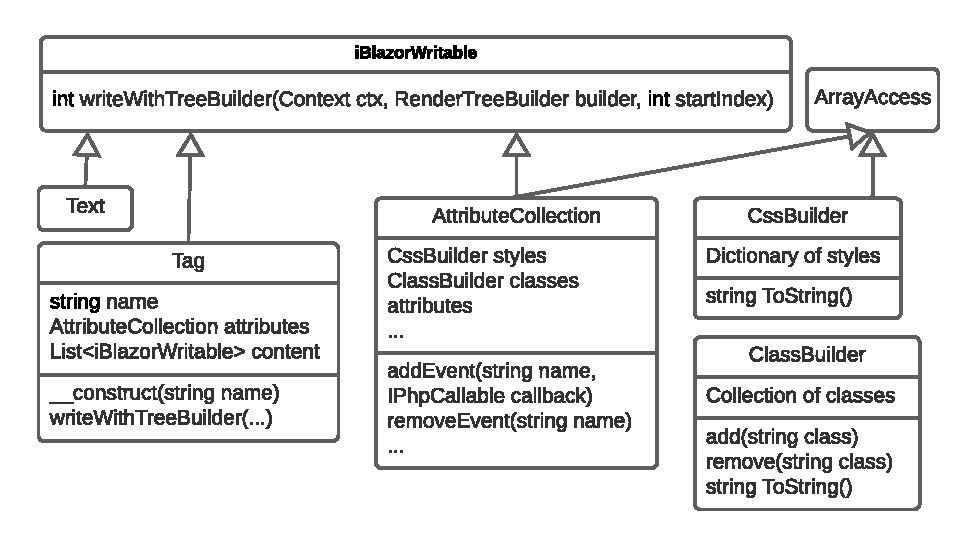
\includegraphics[scale=0.8]{./img/ComponentLibrary}
\caption{Class diagram of supporting library for writting tags.}
\label{img16:diagram}
\end{figure} 
\par
The next barrier is assigning handlers to C\# events in PHP code.
Peachpie does not either support accessing the events.
Thus, we can not directly use a class like \texttt{Timer}, which is useful in the \textit{WebGame} use case for updating the screen every defined period of time.
The issue can be solved by helper methods defined in a C\# static class, \texttt{EventHelper}.
They accept the object providing some events, handler, and event name.
Afterward, we can use reflection for obtaining the desired event by name from the object and then assign the \texttt{IPhpCallable} handler to it.
Because \texttt{Timer} is a common object, we create an additional PHP wrapper class, which uses the timer.
Then a programmer avoids to use the workaround defined above.
\par
The last feature to discuss in this section is interoperability between Javascript and PHP.
As we mentioned, Blazor allows calling Javascript functions from C\# \squarecite{23} and vice-versa \squarecite{24}.
We can utilize a Blazor service,\texttt{IJSRuntime}, injected by the dispatcher, to call Javascript functions.
The service offers a specialized API for that.
Calling PHP from Javascript is more complex.
Peachpie enables calling PHP function by \texttt{Call} method of \texttt{Context}. 
The context finds already defined methods contained in the included PHP script and executes it with the current context.
When we want to call C\# instance method from Javascript, we have to have the reference, supplied by the framework, for calling it.
Additionally, the called C\# method has to be marked with a \texttt{JSInvokableAttribute} during compilation.
The reference can be assigned from C\# by a method, which creates it and uses it as a parameter of a Javascript function.
These conditions lead us to create a new Peachpie context,\texttt{BlazorContext}, which inherits the original Peachpie context and provides the \texttt{CallPHP} method marked by the attribute and calling the PHP function based on parameters.
The context requests the mentioned services provided by the dispatcher and sets the reference by calling predefined code in \texttt{Peachpie.Blazor.js}.
The context will be the Peachpie context of the component.
Thus, it enables to call PHP methods defined in this context from Javascript by using the reference.
The advantage of this approach is that we can have two components inheriting \texttt{PhpComponent} with the same context when we set their context to the same instance.
Thus, we can call their functions by only one reference.
\par
\begin{figure}\centering
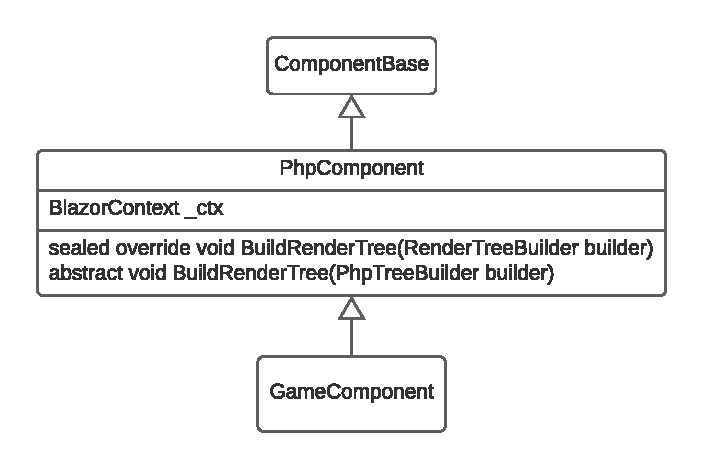
\includegraphics[scale=0.8]{./img/PhpComponentSolution}
\caption{Class diagram of the use case solution.}
\label{img17:solution}
\end{figure}
\par
We summarize the architecture of \texttt{PhpComponent} and solution of \textit{WebGame} use case.
The component hides the original function for rendering and replaces it with our version of the builder, as shown in Figure \ref{img17:solution}.
It results in transparent usage of the builder in the inherited class.
The builder is just a wrapper, so the programmer can use the original builder by accessing its property, \texttt{Builder}.
Additionally, there is a collection of classes for creating tags, making builder usage easier.
For assigning PHP handlers to C\# events, there is a universal helper class, \texttt{EventHelper}.
Furthermore, the last feature is a timer wrapper, which uses the C\# timer, offering a convenient API.
We can use our predefined API using \texttt{BlazorContext} for interoperability with Javascript.
These features are sufficient for implementing a game described in \textit{WebGame} use case.
Using PHP functions as handlers, we use the timer to update the game screen by \texttt{StateHasChanged}.
The update consists of evaluating the position of game entities, which use the helper classes representing HTML entities.
Lastly, we use context preservation to keep the game state.
\par
The last necessary thing is to get assembly references containing the components to \texttt{Router}, which is a standard duty in Blazor.

\section{PhpScriptProvider}

At the beginning of this section, we introduce the main component parts, which gives us an overview of the component composition.
We divide component duties like navigation or script execution into subsections because the component consists of many processes, which are complex to describe at once in the structure.
The component functionality will be explained in these sections.
\par
\begin{figure}[b]\centering
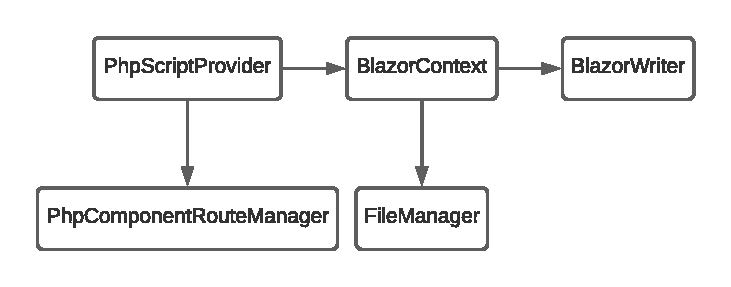
\includegraphics[scale=0.8]{./img/PhpScriptProvider}
\caption{Diagram illustrating usage of PhpScriptProvider main parts.}
\label{img18:provider}
\end{figure}
\par
We start with Figure \ref{img18:provider} describing the connections between the main parts.
\texttt{PhpScriptProvider} is a class, representing a Blazor component.
The component manages the following features.
\par
\begin{itemize}
\item It handles the navigation.
\item It finds the script by name based on provider mode.
\item It creates and keeps a PHP context, which is used for script execution.
\item It executes the script.
\end{itemize}
\par
These duties contain several steps, which are maintained by the helper classes.
As we can see, there is \texttt{PhpComponentRouteManager}, which finds the components, inheriting \texttt{PhpComponent}, based on \texttt{RouteAttribute}.
It enables navigation of Blazor components defined in PHP scripts.
The next part is \texttt{BlazorContext} already mentioned in PhpComponent, which is Peachpie \texttt{Context} designed for Blazor enviroment.
The context constructor accepts several Blazor services like \texttt{IJSRuntime} enabling interoperability with Javascript.
The context initializes superglobals based on URL and submitted forms, manages files uploaded by a form, and controls  \texttt{BlazorWriter} which redirects the script output to the render tree.
Lastly, \texttt{FileManager} reads submitted files, downloads them, or deletes them from Browser memory.
\par
We zoom in on \texttt{PhpScriptProvider} structure in order to better understand processes maintaining the features.
The provider contains of many properties.
Some of them are injected by the dispatcher like \texttt{NavigationManager} or \texttt{IJSRuntime}, which is a service providing interoperability with Javascript.
Others can be parametrized, like \texttt{Type} determining the mode of provider, \texttt{ContextLifetime} determining the persistency of the script context, or \texttt{ScriptName} determining the executing script when the mode \textit{Script} is set.
These properties influence the component methods.
The first method is \texttt{Attach}, which assigns a render handle providing \texttt{RenderTreeBuilder}, and registers a navigation handler creating the context and calling \texttt{Refresh}.
The second method,\texttt{SetParameters}, handles calling \texttt{Refresh}, and creating the context as well.
\texttt{Refresh} finds a script or a component based on properties, assigns the superglobals, and calls \texttt{Render} which renders the component or executes the script.
\texttt{OnAfterRender} cares about enabling the forms to send data back to Blazor.
Some of these methods are called by Blazor framework providing the component lifecycle.

\subsection{Navigation}

Now, we explain navigation in \texttt{PhpScriptProvider} for each of its modes.
We have to clarify how the component is instantiated and maintained by Blazor.
There are two ways how to use the component.
The first of them is to set it in \texttt{WebAssemblyBuilder} as a root component,
which is rendered after the first application launch in Blazor.
The component is alive for the whole application life because there is no \texttt{Router}, which disposes components representing a previous page. 
It results in calling the \texttt{Attach} method and the \texttt{SetParameters} method only once.
The second way is to use a Razor page containing the component and let the navigation to the page on \texttt{Router}, which is a root component by default.
When the page is navigated, the component is instantiated as well.
The difference is the possibility of calling the \texttt{SetParameters} method multiple times when the page is parameterized.
Then, when the parameters are changed, Blazor automatically calls the inner component \texttt{SetParameters} methods if the components have at least one complex type. 
This fact is because the Blazor framework can not decide if the parameters, which are complex types, were changed.
\par
The \textit{Router} mode is designed to be used when the component is a root component.
Then we are sure, that \texttt{Attach} and \texttt{SetParameters} methods are called only once.
Thus, we register navigation handler in the \texttt{Attach} method, which should handle further navigation.
When the navigation occurs, we create a new context if the context should not be persistent and call \texttt{Refresh}.
We create a new context and call \texttt{Refresh} method in \texttt{SetParameters} as well, but the method is called only once at the beginning of the application.
Then the \texttt{Refresh} method parses the query part of URL \squarecite{26}, obtained from \texttt{NavigationManager} and gets the script name from the URL.
When we determine the script name, we call the \texttt{Render} method, where we decide if it is a script or a component defined in a script based on \texttt{.php} extension.
If the extension is missing, we try to find a component defined in scripts, which has correct \texttt{RouteAttribute} by \texttt{PhpComponentRouteManager}.
Otherwise, we ask the Peachpie context for obtaining the script representation as \texttt{ScriptInfo}.
Additional manager duty is to assign assembly references containing scripts, to the context, at the beginning of the application.
The context does not have to know the script name, or the component does not have to exist. 
Then we render predefined \textit{not found} page, which can be set by \texttt{PhpScriptProvider} parameters.
Otherwise, we render the script or the component.
Additionally, when we navigate the component, we set its context by our context.
It results in using the interoperability by either provider or the component because we can use the same context reference in Javascript code.
\par
Next modes, \textit{ScriptProvider} and \textit{Script}, are similar.
They are defined in a Razor page and initialized when the page is navigated.  
The difference is finding the script by name, where the \textit{Script} always uses the name defined in the component parameter and \textit{ScriptProvider} finds script based on URL.
As we said, the \texttt{SetParameters} can be called multiple times, so we call \texttt{Refresh} only by the first time in the method.
Additional rendering is initiated by the navigation handler.
Thus, when the navigation occurs, we find and update the page, or the component is disposed if \texttt{Router} matches another Razor page.
We create the new context based on the \texttt{ContextLifetime} mode.
It differs from common PHP behavior, where the context is disposed after scritps handles the request.
This unusual approach allows calling functions defined in the context after the component is rendered, which is a part of Javascript interoperability when we can call PHP functions by Javascript.
We should check if the component has not already been disposed by \texttt{Router} before calling the \texttt{Refresh}.
Obtaining the script is similar to \textit{Router} mode.

\subsection{Script Execution}
We start with \texttt{BlazorWriter}, which inherits \texttt{TextWriter}.
The inheritance allows using the writer as \texttt{BlazorContext} output writer, which manipulates with script output.
The writer consists of a buffer and \texttt{RenderTreeBuilder}.
The main usage is to write any string to the writer, which adds it to the buffer.
In the end, the writer flushes it into the builder by \texttt{AddMarkUpContent}.
It results in treating the whole script output as one modification by diff algorithm, which causes the whole page update instead of smaller necessary updates.
This approach is chose due to the following limitations.
\texttt{AddMarkUpContent} does not allow to add incomplete markup text, meaning that tags are not properly closed.
Thus, we can not divide the text into smaller parts because of the HTML nature, where tags are coupled by other tags.
The second possibility is to parse the output and recognize the types of HTML entities, which can use specialized builder API.
However, it is not suitable because of parser complexity.
It is important to dispose the writer after the rendering because the same builder can not be repeatedly used.
\par
\texttt{BlazorContext} maintains the writer and interoperability with Javascript.
It provides methods for initializing and ending the rendering.
The script represented by \texttt{ScriptInfo} is executed by its method \texttt{Evaluate}. This method accepts the context, which maintains the script output by redirecting it to the render tree.
It also allows setting superglobals like \texttt{\$\_GET} to provide the query part of URL and turns forms to client-side 
handling, which is described in the following section.

\subsection{Forms}

Typically, web forms are not handled by Blazor, and the are sent to the server.
We use Javascript interoperability to evaluate them on the client side.
It starts in \texttt{AfterRender} method, where we call our Javascript function, which finds all already rendered forms and assigns them an event handler for submitting.
When submit occurs, the handler collects all data from the form, does ordinary navigation to the page defined in \texttt{action} attribute, and prevents default behavior, which is sending the form to the server.
When the navigation is handled by \texttt{PhpScriptProvider}, it gets all collected data and assigns the context superglobals by them.
Afterward, the script is executed, and it can access the superglobals.
\par
In the previous paragraph, we did not explain the file management due to its complexity.
We describe it now.
When a user loads files by form, Javascript obtains only the list of files. 
When we want to read the content, we have to use a reading operation, which is done asynchronously by \texttt{Promise} mentioned in the Javascript section.
Thus, when we get the data during navigation, we have to wait until the content is read.
This operation could take a long time, so the page shows old content.
For this reason, we provide an additional parameter for defining the content, which is shown during navigation.
An alternative is initializing reading by a PHP script when it is executed.
It uses interoperability between PHP, C\#, and Javascript in order to call desired reading methods.
Unfortunately, Blazor does not allow us to wait until the reading operation is done, and we have to provide callbacks, which handle the end of the reading.
We suppose that it is confusing for potential PHP programmers, who will use our solution to define PHP callbacks.
We decide to prefetch the file content before the execution to provide the data synchronously in PHP code.
\par
Interoperability in the provider can be achieved in a similar manner as in \texttt{PhpComponent}.
The difference is calling the Javascript functions, which use prefined API using our context, which uses the \texttt{IJSRuntime} service.


            
 
\chapter{Examples}

This chapter demonstrates the usage of our solution by four examples, which are inspired by the use cases mentioned earlier.
We describe example structure, show important blocks of code, which has to be added to project.
At the end, we make snapshots of the websites.
\par

\section{WebGame}

The example aims at the third use case.
It contains a game where we have a rocket, which has to destroy falling asteroids with bullets, as we can see in Figure \ref{img28:game}.
We can also see current \ac{FPS} in the left corner of the screenshot.
The rocket can be control by buttons in the bottom, or we can use a keyboard, where arrows determine the rocket movement and \texttt{F} key fires a bullet.
We will discuss the rendering time in the benchmark section.
\par
\begin{figure}\centering
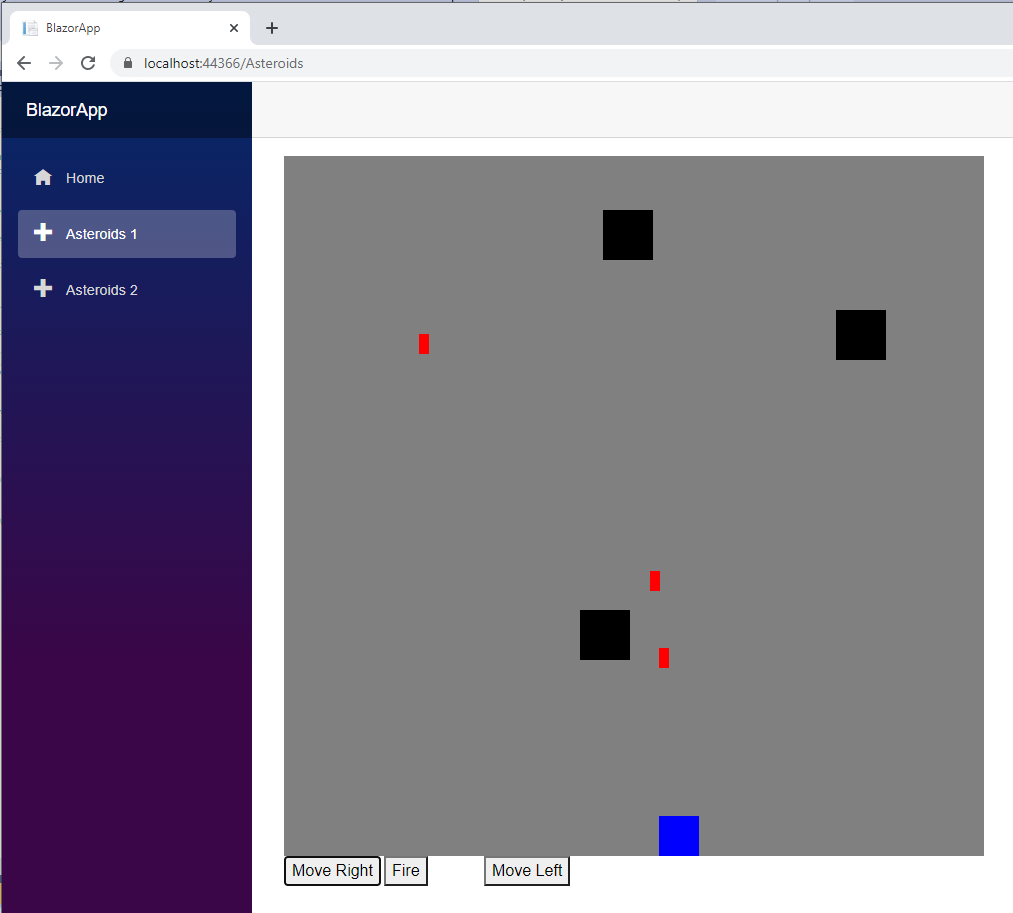
\includegraphics[scale=0.5]{./img/Asteroids}
\caption{The game.}
\label{img28:game}
\end{figure} 
\par
The example is implemented as .NET solution consisting of three projects. 
\texttt{BlazorApp.Client} and \texttt{BlazorApp.Server} are pregenerated projects by the Blazor App template.
The game is implemented in the Peachpie \texttt{PHPScripts} project.
These projects reference the \texttt{Peachpie.Blazor} library as a NuGet package containing our solution. 
We describe steps, which was necessary for making the game working.
\par
The game implementation is contained in three PHP scripts and a CSS file containing game styles.
The \textit{settings.php} script contains default values of FPS, an asteroids frequency, and additional settings.
The \textit{asteroids.php} script contains definitions of game entities like the rocket or an asteroid.
These entities utilizes \texttt{Peachpie.Blazor} library, which provides helper classes representing HTML elements.
At the bottom of the script is \texttt{Application} class connecting all parts together.
The class uses HTML elements events for interacting with the user due to the \texttt{PhpTreeBuilder} class providing an API targeting PHP usage.
The last script is \textit{main.php}, which contains \texttt{AsteroidsComponent} class.
This class is routable by \texttt{/Asteroids} URL and initializes the game.
It uses \texttt{Timer} provided by \texttt{Peachpie.Blazor}, which enables to handles tick events, which update the game and the screen.
Because \texttt{Application} class inherits the helper class \texttt{Tag}, \texttt{AscteroidsComponent} does not bother with game rendering and uses \texttt{BlazorWritable} interface for transparent initiating the rendering.
\par
\texttt{BlazorApp.Client} references the game and uses the default \texttt{Router} component to navigate \texttt{AsteroidsComonent}.
\texttt{index.html} contains links to the game styles and a supporting Javascript defined in the \texttt{Peachpie.Blazor} library.
We can see two examples of \texttt{AsteroidsComponent} usage in Figure \ref{img28:game}.
\textit{Asteroids 1} utilizes the router for navigating it.
\textit{Asteroids 2} utilizes a Razor page, which contains additional content with the game.
\par
\texttt{BlazorApp.Server} provides the Web Static Assets to a client by inserting additional middlewares, which handles their requests.
This insertion can be seen in the \textit{Startup.cs} file and in Figure \ref{img21:server}.
The website is run by launching the server.
\par
\begin{figure}
\begin{lstlisting}
var fileProvider = new ManifestEmbeddedFileProvider(
	typeof(PhpBlazor.BlazorContext).Assembly);
app.UseStaticFiles(new StaticFileOptions() {
	 FileProvider = fileProvider });

app.UseStaticFiles(new StaticFileOptions
{
	FileProvider = new PhysicalFileProvider(
		Path to static resources, "PHPScripts\\wwwroot")),
	RequestPath = "/Asteroids"
});
\end{lstlisting}
\caption{A part of the \texttt{Configure} method contained in the \texttt{StartUp} class, which is defined in \textit{Startup.cs}}
\label{img21:server}
\end{figure}

\section{Web}

Web example is inspired by the first use case, which moves the website on a client side.
The website contains a simple layout consisting of references to the website parts.
We can see the default page in Figure \ref{img28:website}.
The website contains images, which are downloaded from the server when they are required.
\par
\begin{figure}[!b]\centering
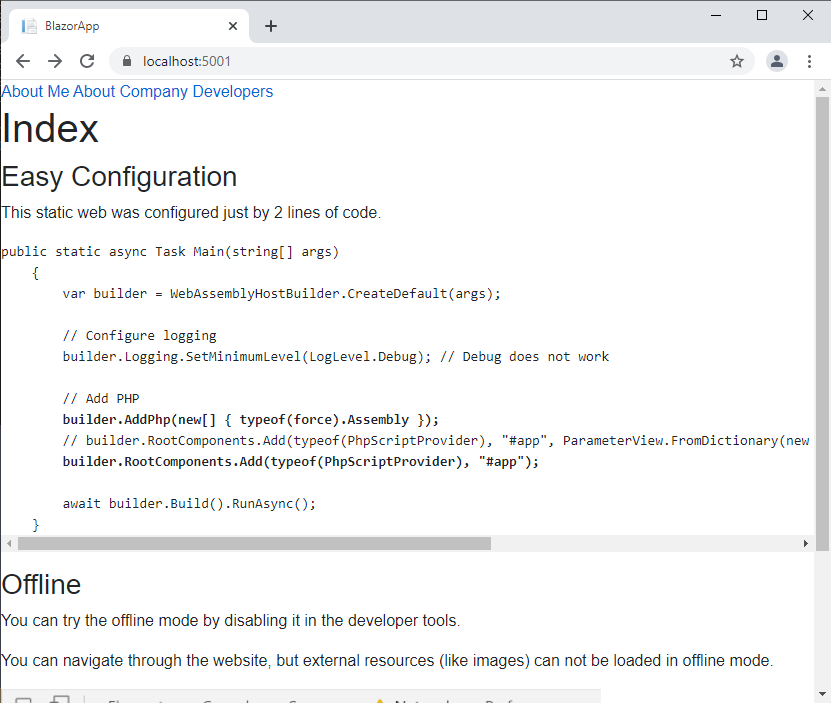
\includegraphics[scale=0.5]{./img/Web}
\caption{The default page.}
\label{img28:website}
\end{figure} 
\par
The whole application is implemented as .NET solution consisting of three projects.
\texttt{BlazorApp.Client} represents the client application containing \texttt{Program.cs}, which sets \texttt{WebAssemblyBuilder} with a root component, \texttt{PhpScriptProvider}, as we can see in Figure \ref{img20:program}.
\texttt{Blazor.Server} has the same role as in the previous example.
\par
\begin{figure}
\begin{lstlisting}
public static async Task Main(string[] args)
{
	var builder = WebAssemblyHostBuilder.CreateDefault(args);

	// Configure logging
	builder.Logging.SetMinimumLevel(LogLevel.Debug);

	// Add PHP
	builder.AddPhp(new[] { typeof(force).Assembly });
	builder.RootComponents.Add(typeof(PhpScriptProvider), "#app");
            
	await builder.Build().RunAsync();
}
\end{lstlisting}
\caption{The Main method in Program.cs}
\label{img20:program}
\end{figure}
\par
The project references \texttt{Peachpie.Blazor} library and the Peachpie project, \texttt{PHPScripts}, containing PHP scripts representing the website.
The provider has default settings, which are the \texttt{Router} type and the \texttt{OnNavigationChanged} mode of \texttt{BlazorContext}.
Furthermore, we have to link the Javascript script from \texttt{Peachpie.Blazor} library to \textit{index.html} in order to use it during the runtime.
\par
The \texttt{PHPScripts} project contains the programmer's defined PHP scripts forming the web of some software company.
We can see the project content in Figure \ref{img22:web}.
The project uses Peachpie \ac{SDK} for compiling the scripts.
The website has a simple layout defined in \textit{defaultLayout.php} referencing pages about the founder, the company, and the community.
The \textit{me.php} page contains an image, \textit{logo.png}, which is loaded by a common tag, \texttt{<img alt="Logo" src="Web/images/logo.png"/>}.
We can see the \textit{force.php} script containing empty \texttt{force} class, which is used in \texttt{BlazorApp.Client} to force loading of this assembly to a client.
\par
\begin{figure}\centering
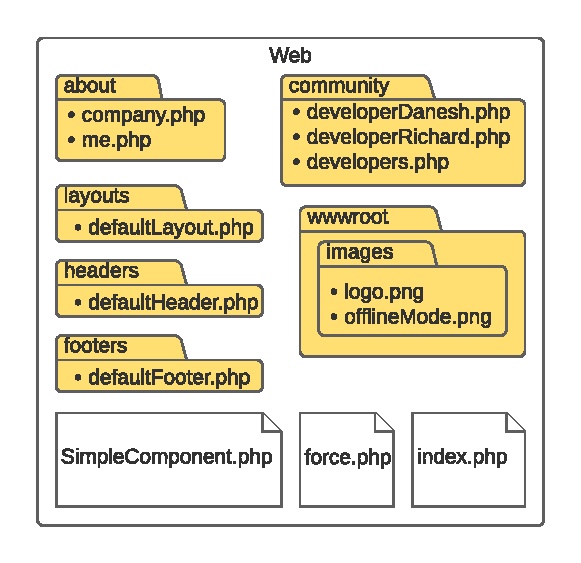
\includegraphics[scale=0.9]{./img/WebStructure}
\caption{The Web solution structure.}
\label{img22:web}
\end{figure} 
\par
An interesting page is \textit{developers.php}, which displays information about developers working in the company.
We can see the script in Figure \ref{img25:developer}
It uses script inclusion to add the head section.
Then, there is a Javascript call, which uses our predefined API, which causes showing the alert with the message when the page loads.
The whole page uses HTML interleaving.
We can see using \texttt{\$\_GET} superglobal in the script, where we decide to show its content based on the URL query.
When we have the \textit{OnNavigationChanged} mode for the context, and we refresh the page after navigation to a developer, then we can see the anchors to developers.
It is caused by creating a new context between navigation, so the variables are disposed.
With the second mode of context,\texttt{Persistant}, we still have the info page of the firstly navigated developer because the variables in the context remain.
This page is transparently rendered by our \texttt{PhpScriptProvider}, which evaluates the whole script and adds the output as a markup text to the builder.
\par
\begin{figure}
\begin{lstlisting}
<?php
    require("/headers/defaultHeader.php");
    CallJsVoid("window.alert", "Hello from PHP script.");
?>
<?php
if (isset($_GET["developer"])) { 
    $name = $_GET["developer"];
    require("/community/developer$name.php");
} else {
?>
...
<p>Get more info about 
<a href="/community/developers.php?developer=Richard">Richard</a>.
</p>
...
<?php } ?>
<?php
    require("/footers/defaultFooter.php");
?>
\end{lstlisting}
\caption{developers.php}
\label{img25:developer}
\end{figure}

\section{OneScript}

In this example, we aim at the second use case.
The website contains several pages with demonstrates inserting page fragments written in PHP to the Blazor website.
When we navigate the page, we can see a button, which utilizes interoperability between PHP and Javascript provided by our solution.
When we click on it, the javascript code calls PHP code, which writes a message to a browser console.
Next examples referred as \textit{Example 1}, \textit{Example 2}, \textit{Example 3} show working with forms.
The first example uses a simple form with the \texttt{GET} method.
When we submit the form, we are navigated to a page written in PHP, displaying the content of superglobals.
The same process is done with the \texttt{POST} method.
We can also try to load a file to the form in the last example.
After the submit, the page displays its file contect encoded into \textit{base64} encoding.
\textit{Example 4} uses previously mentioned features to enable displaying user defines graphs.
We can upload a file containing the graph, or the application will generate it.
Then the graph is displayed, and we can download the points defining it as we can see in Figure \ref{img27:graph}.
\par
\begin{figure}\centering
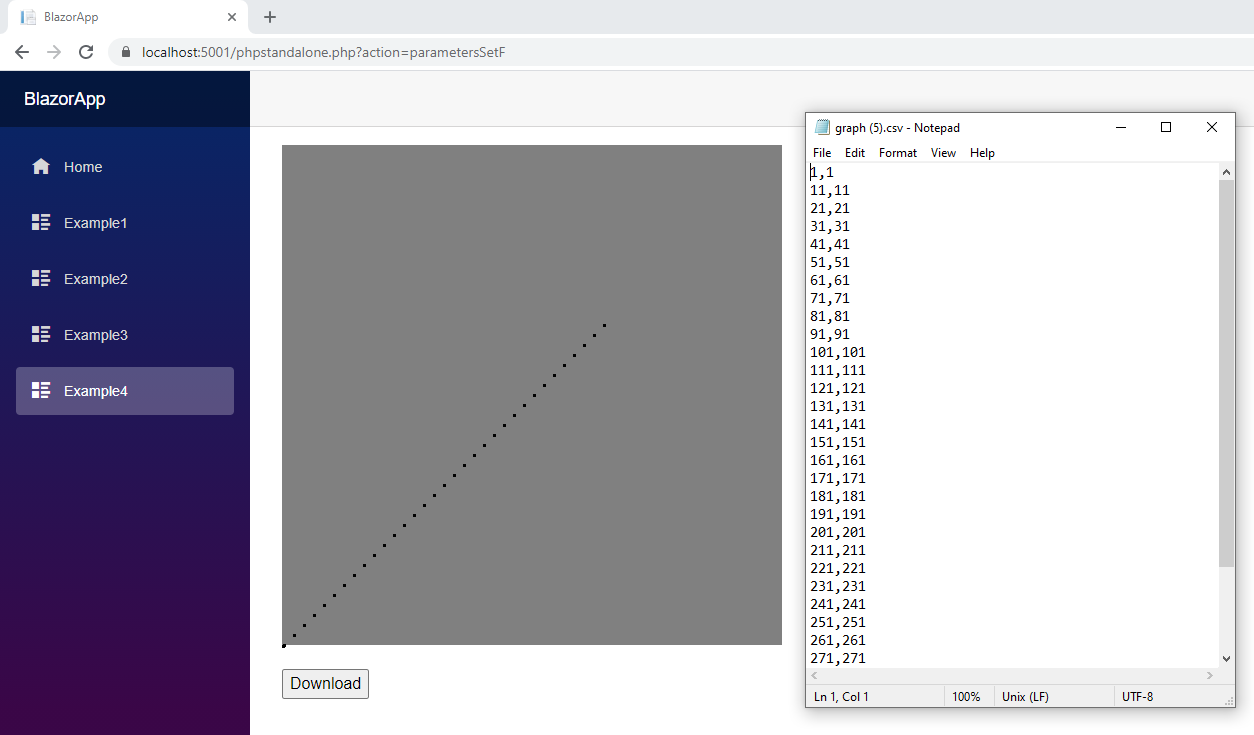
\includegraphics[scale=0.4]{./img/graph}
\caption{Application for visualising a graph.}
\label{img27:graph}
\end{figure} 
\par
The .NET solution consists of three projects.
\texttt{BlazorApp.Server} is the same as previois ones.
\texttt{BlazorApp.Client} contains common Razor pages, and has default \texttt{Router} as a root component.
We create several scripts in the Peachpie\texttt{PHPScripts} project to enrich the website with all content except the layout, which we presented.
The website contains three Razor pages: \textit{Index.razor}, \textit{PhpGateway.razor}, and \textit{PhpScript.razor}.
The first page uses \texttt{PhpScriptProvider} to navigate \texttt{index.php}.
Using the provider is straightforward.
\par
We want to show the calling PHP function from Javascript in Figure \ref{img26:index}.
As we can see, it is effortless to call it.
The \texttt{callPHP} function accepts the function name and object to serialize as an function parameter.
When the script is rendered, the context contains defined \texttt{CallPHP} function.
We click on the button, which invokes \texttt{Call} method on the context, which invokes the desired function.
Then, we deserialize the parameter.
There is an interesting thing about using \texttt{echo}, \texttt{print}, etc. when the script is not rendered.
The context provides the second writer, which uses \texttt{Console} as the output.
It causes printing the message into the web browser console.
\begin{figure}
\begin{lstlisting}
...
<p>Click and look at console output</p>
<button onclick="window.php.callPHP('CallPHP',
	{ name : 'Bon', surname: 'Jovi'});">PHP</button>
<?php

function CallPHP($data)
{
    $json = json_decode($data); 

	echo "Hello " . $json->name . " ";
	echo $json->surname .  " from PHP\n";
}
\end{lstlisting}
\caption{\textit{index.php}}
\label{img26:index}
\end{figure}
\par
Another part of the website uses forms to demonstrates \texttt{GET} and \texttt{POST} method.
We can see it in \textit{php} folder, where are three examples of forms using both methods and file loading.
These examples can be navigated based on their names due to the unspecified URL of the Razor page, which uses the provider.
After navigation to this page, the provider gets the script name from the URL.
\par
The graph visualization aims at the persistent context and using forms as interaction with the user.
It is a common approach in PHP, and we can use it on a client side due to our solution.
There is a simple application enabling us to visualize a graph, as we can see in the folder \texttt{fileManagement}.
The application can upload a CSV file containing a graph or generate a new one based on the given parameters.
We use PHP library for parsing the file, which demonstrates a possibility to utilize the already created library on a client side.
The application has the main script,\texttt{fileManagment/index.php}, which recognizes what to do based on superglobals and saved variables.
It is possible due to context persistence.

\section{AllTogether}

This example aims at the fourth use case, where we want to connect PHP and C\# to form one website.
It uses the website made in the first example and includes it in the already existing Blazor website.
It connects the game created earlier and the graph visualizer to show context sharing between \texttt{PhpScriptProvider} and \texttt{PhpComponent}.
We can see the default page of the PHP website in Figure \ref{img30:allTogether}.
The game can be navigated by an anchor, \texttt{Start}.
When we play it, we can restart it with an anchor placed above the game.
Afterward, we can see a graph, which contains a score generated by the game. 
\par
\begin{figure}\centering
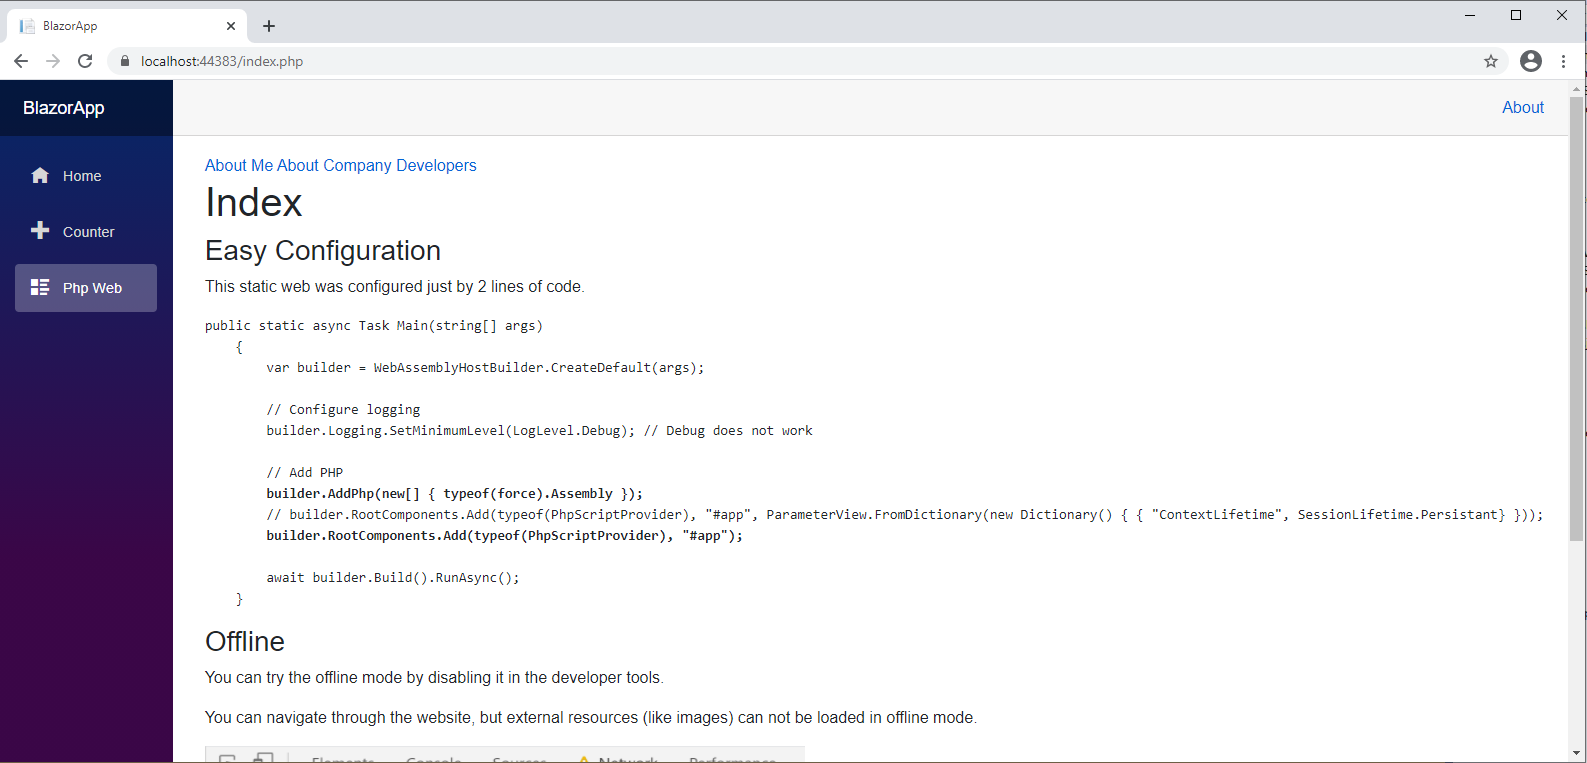
\includegraphics[scale=0.5]{./img/AllTogether}
\caption{The example.}
\label{img30:allTogether}
\end{figure} 
\par
The .NET solution again contains three projects \texttt{BlazorApp.Client}, \texttt{BlazorApp.Server}, and \texttt{PHPScripts}.
\texttt{PHPScripts} consists of \textit{Game}, \textit{Graph}, \textit{Web}, and \textit{wwwroot} folders.
We already know the implementation of these parts.
An interesting collaboration is between the game and the graph, where we save a global variable containing the graph in \texttt{AsteroidsComponent} and uses later in \textit{main.php} script of graph visualization.
This works due to \texttt{PhpScriptProvider}, where we navigate either the \textit{main.php} or \texttt{AsteroidsComponent}.
Because the context can be persistent, we share global variables between these parts, and we can communicate through them.
We choose between navigated parts by a submit form containing one button, which navigates to the game, and an anchor containing a reference to the \textit{main.php}.
Because the default \texttt{Router} can navigate the \texttt{AsteroidsComponent}, we don't add the \texttt{PHPScripts} assembly to the router additional assemblies in order to keep the provider alive and share its content with the game.
\par
\texttt{BlazorApp.Client} contains the \textit{Web.razor} page containg \texttt{PhpScriptProvider}, which manages the PHP website navigation.
It contains the \texttt{Game.razor} page, which is shown in Figure \ref{img29:razor}.
There is a trick with the navigation.
Because the default Blazor \texttt{Router} is a root component, it reacts to navigation, but we want to navigate the game and graph visualization by the provider.
This can be avoided by defining two routable paths, which navigate the same Razor page, but the different content by our provider.
\par
\begin{figure}[!b]
\begin{lstlisting}
@page "/Graph/index.php"
@page "/Asteroids"
@using Peachpie.Blazor

<PhpScriptProvider ContextLifetime="@SessionLifetime.Persistant" 
Type="@PhpScriptProviderType.ScriptProvider">
    <Navigating>
        <p>Navigating</p>
    </Navigating>
    <NotFound>
        <p>Not found</p>
    </NotFound>
</PhpScriptProvider>
\end{lstlisting}
\caption{\textit{Game.razor}}
\label{img29:razor}
\end{figure}

\chapter{Benchmarks}

In this chapter, we present two benchmarks, which explore the used technology limitations.
We introduce the background of the benchmarks, execute them and then evaluate the results.

\section{Rendering}

\section{GD library}

This benchmark tests the effectivity of PHP library, \textit{gdlibrary}, in the Blazor environment.
We prepare a simple script, which creates a blank image with 1920x1080 resolution.
We use \texttt{imagecreatetruecolor} function defined in the library.
Then we measure elapsed time during the function execution by printing the current time before and after the function call.
We compare the results with executing the script in desktop environments, where we use Peachpie and native PHP interpreter.
\par
\begin{table}
\centering
\begin{tabular}{l@{\hspace{1.5cm}}D{.}{,}{3.2}D{.}{,}{1.2}D{.}{,}{2.3}}
\toprule
\mc{\textbf{Enviroment}} & \mc{\textbf{Execution time}}\\
\midrule
Blazor   & \mc{---} \\
Peachpie & \mc{---} \\
Native   & \mc{---} \\
\end{tabular}
\caption{Elapsed time of the function execution.}
\label{tab01:time}
\end{table}
\par
We can see measured data in Table \ref{tab01:time}.


\chapter*{Conclusion}
\addcontentsline{toc}{chapter}{Conclusion}

\section*{Future work}
\addcontentsline{toc}{section}{Future work}

%%% Bibliography
%%% Bibliography (literature used as a source)
%%%
%%% We employ bibTeX to construct the bibliography. It processes
%%% citations in the text (e.g., the \cite{...} macro) and looks up
%%% relevant entries in the bibliography.bib file.
%%%
%%% The \bibliographystyle command selects, which style will be used
%%% for references from the text. The argument in curly brackets is
%%% the name of the corresponding style file (*.bst). Both styles
%%% mentioned in this template are included in LaTeX distributions.

\bibliographystyle{plainnat}    %% Author (year)
% \bibliographystyle{unsrt}     %% [number]

\renewcommand{\bibname}{Bibliography}

%%% Generate the bibliography. Beware that if you cited no works,
%%% the empty list will be omitted completely.

\bibliography{bibliography}

%%% If case you prefer to write the bibliography manually (without bibTeX),
%%% you can use the following. Please follow the ISO 690 standard and
%%% citation conventions of your field of research.

% \begin{thebibliography}{99}
%
% \bibitem{lamport94}
%   {\sc Lamport,} Leslie.
%   \emph{\LaTeX: A Document Preparation System}.
%   2nd edition.
%   Massachusetts: Addison Wesley, 1994.
%   ISBN 0-201-52983-1.
%
% \end{thebibliography}


%%% Figures used in the thesis (consider if this is needed)
\listoffigures

%%% Tables used in the thesis (consider if this is needed)
%%% In mathematical theses, it could be better to move the list of tables to the beginning of the thesis.
\listoftables

%%% Abbreviations used in the thesis, if any, including their explanation
%%% In mathematical theses, it could be better to move the list of abbreviations to the beginning of the thesis.
\chapwithtoc{List of Abbreviations}

%%% Attachments to the bachelor thesis, if any. Each attachment must be
%%% referred to at least once from the text of the thesis. Attachments
%%% are numbered.
%%%
%%% The printed version should preferably contain attachments, which can be
%%% read (additional tables and charts, supplementary text, examples of
%%% program output, etc.). The electronic version is more suited for attachments
%%% which will likely be used in an electronic form rather than read (program
%%% source code, data files, interactive charts, etc.). Electronic attachments
%%% should be uploaded to SIS and optionally also included in the thesis on a~CD/DVD.
%%% Allowed file formats are specified in provision of the rector no. 72/2017.
\appendix
\chapter{Attachments}

\section{First Attachment}

\openright
\end{document}
